\documentclass[11pt,a4paper]{article}

% ─── Packages ────────────────────────────────────────────────────────────────
\usepackage[margin=2.5cm]{geometry}
\usepackage{amsmath, amssymb, bm}
\usepackage{graphicx}
\usepackage{booktabs}
\usepackage[dvipsnames,svgnames,table]{xcolor}
\usepackage{hyperref}
\usepackage{subcaption}
\usepackage{tikz}
\usetikzlibrary{arrows.meta, positioning, shapes.geometric, calc}
\usepackage{cleveref}
\usepackage{listings}

\usepackage{float}
\usepackage{caption}
\usepackage{parskip}
\setlength{\parskip}{0.5em}

\hypersetup{colorlinks=true, linkcolor=blue!70!black, citecolor=green!50!black,
            urlcolor=blue!60!black}

\definecolor{red3}{RGB}{214,39,40}
\definecolor{blue2}{RGB}{31,119,180}
\definecolor{orange2}{RGB}{255,127,14}
\definecolor{gray1}{RGB}{100,100,100}
\definecolor{codeblue}{RGB}{0,0,180}
\definecolor{codegray}{RGB}{128,128,128}

\lstset{
  basicstyle=\ttfamily\small,
  keywordstyle=\color{codeblue},
  commentstyle=\color{codegray}\itshape,
  stringstyle=\color{red!60!black},
  breaklines=true,
  frame=single,
  numbers=left,
  numberstyle=\tiny\color{gray},
  xleftmargin=1.5em,
  language=Python,
}

\captionsetup{font=small, labelfont=bf}

% ─── Macros ──────────────────────────────────────────────────────────────────
\newcommand{\pinv}[1]{#1^{\dagger}}
\newcommand{\R}[1]{\mathbb{R}^{#1}}
\newcommand{\bJ}{\bm{J}}
\newcommand{\btau}{\bm{\tau}}
\newcommand{\bq}{\bm{q}}
\newcommand{\bF}{\bm{F}}
\newcommand{\bw}{\bm{w}}
\newcommand{\btheta}{\bm{\theta}}
\newcommand{\re}[1]{\textcolor{red3}{\textbf{#1}}}
\newcommand{\good}[1]{\textcolor{blue2}{\textbf{#1}}}

% ─── Title ───────────────────────────────────────────────────────────────────
\title{\textbf{Root Cause Analysis: RE3 Deployment Disaster}\\[0.4em]
       \large Jacobian Amplification of Structural Dynamics in\\
       Pinocchio-based Wrench Estimation}
\author{H1.2 Adaptive Policy Team}
\date{2026-03-16}

% ─────────────────────────────────────────────────────────────────────────────
\begin{document}
\maketitle
\tableofcontents
\newpage

% ═════════════════════════════════════════════════════════════════════════════
\section{Abstract}
% ═════════════════════════════════════════════════════════════════════════════

During episode \texttt{re3\_real\_encode\_tr1}, an RL balancing policy
deployed on the H1.2 humanoid robot caused violent involuntary leg
thrashing within 0.16 seconds of engagement, ultimately producing hip-pitch
torques exceeding 428 N$\cdot$m.  The robot was stopped before structural
damage occurred.

This document provides a ground-up technical analysis of the root cause.
We cover: (1) a first-principles introduction to rigid-body dynamics
and the Pinocchio framework; (2) the mathematics of estimating an external
wrench from internal motor torques via the Jacobian pseudo-inverse; (3) why
an ill-conditioned Jacobian amplifies any upstream torque residual into a
spurious end-effector force; (4) a step-by-step numerical reconstruction of
the cascade from policy steps 0--8; and (5) a revised causal hypothesis that
inverts the previously posted narrative.

\medskip
\noindent\textbf{Revised hypothesis (confirmed by data):}
\begin{enumerate}
\item In RE3, the left arm was in the \texttt{arm\_waist\_target} pose
      (shoulder pitched $-17°$ from motor zero, elbow extended $86°$ from
      motor zero), which physically corresponds to the arm hanging
      \emph{straight down and limp} alongside the torso.  In RE1/RE2 the
      arms were at motor zero, physically corresponding to forearms
      bent at the sides.  The extended/limp left arm created a
      \textbf{15.6$\times$ torso$\to$wrist-$F_z$ Jacobian amplification}.
\item Both \re{RE3} and \good{RE2} began with similar large hip-roll
      position errors ($\sim$0.35--0.51 rad).  The initial leg dynamics
      were comparable, but RE3's ill-conditioned Jacobian turned normal
      torso structural torques into catastrophic phantom wrist forces.
\item The structural torque required by the torso motor to counteract leg
      dynamics was indistinguishable from normal, but with a 15.6$\times$
      amplification it produced a $-533$ N spurious left wrist force.
\item The policy interpreted this as a large external push at the wrist and
      commanded increasingly extreme leg targets, driving the torso torque
      higher, completing a positive feedback loop.
\end{enumerate}

% ═════════════════════════════════════════════════════════════════════════════
\section{Background: Pinocchio and Rigid-Body Dynamics}
% ═════════════════════════════════════════════════════════════════════════════

\subsection{What is Pinocchio?}

Pinocchio~\cite{pinocchio} is an open-source rigid-body dynamics library
that operates on a robot model loaded from a URDF file.  It represents the
robot as a \emph{kinematic tree}: a directed graph of rigid bodies
(\emph{links}) connected by joints.  For the H1.2 we use a free-flyer root
joint (6-DOF floating base) plus 27 actuated joints (legs, torso, arms),
giving a configuration space of dimension $n_q = 34$ (7 free-flyer
coefficients + 27 joint angles) and velocity space $n_v = 33$.

The library provides:
\begin{itemize}
\item \textbf{Forward kinematics} (\texttt{forwardKinematics}): given
      $\bq$, compute the pose of every link/frame.
\item \textbf{Recursive Newton-Euler Algorithm} (\texttt{rnea}):
      compute the joint torques $\btau$ required to achieve a given
      $(\bq, \dot\bq, \ddot\bq)$, including gravity.
\item \textbf{Frame Jacobian} (\texttt{computeFrameJacobian}): the matrix
      $\bJ \in \R{6 \times n_v}$ mapping joint velocities to the
      6-D twist (linear+angular velocity) of a specific link frame.
\end{itemize}

\subsection{The Robot Configuration Vector}

The 27 actuated joints are ordered as shown in
Table~\ref{tab:joint_order}.  All data arrays (\texttt{tau.npy},
\texttt{qpos.npy}, \texttt{target\_dof.npy}) use this ordering.

\begin{table}[H]
\centering
\caption{Joint index ordering in 27-column arrays.}
\label{tab:joint_order}
\begin{tabular}{rll}
\toprule
Indices & Group & Joints \\
\midrule
0--5  & Left leg  & l\_hip\_yaw, l\_hip\_pitch, l\_hip\_roll, l\_knee, l\_ank\_pitch, l\_ank\_roll \\
6--11 & Right leg & r\_hip\_yaw, r\_hip\_pitch, r\_hip\_roll, r\_knee, r\_ank\_pitch, r\_ank\_roll \\
12    & Torso     & torso \\
13--19 & Left arm  & L\_sh\_pitch, L\_sh\_roll, L\_sh\_yaw, L\_elbow, L\_wr\_roll, L\_wr\_pitch, L\_wr\_yaw \\
20--26 & Right arm & R\_sh\_pitch, R\_sh\_roll, R\_sh\_yaw, R\_elbow, R\_wr\_roll, R\_wr\_pitch, R\_wr\_yaw \\
\bottomrule
\end{tabular}
\end{table}

\subsection{Forward Kinematics and the Frame Jacobian}

Given a configuration $\bq$, forward kinematics computes the homogeneous
transform $T^{w}_{f}(\bq) \in SE(3)$ from the world frame to any target
frame $f$.  For the \emph{left wrist yaw link}:
\begin{equation}
  T^{w}_{\text{lwrist}}(\bq) = T^{w}_{\text{pelvis}} \cdot
  T^{\text{pelvis}}_{\text{torso}} \cdot
  T^{\text{torso}}_{\text{L\_sh\_pitch}} \cdots
  T^{\text{L\_elbow}}_{\text{lwrist}},
\end{equation}
where each factor depends only on the joint angles along the kinematic chain.

The \emph{geometric Jacobian} of frame $f$ in the
LOCAL\_WORLD\_ALIGNED convention is the $6 \times n_v$ matrix:
\begin{equation}
  \bJ_f(\bq) \triangleq
  \frac{\partial}{\partial \bq}
  \begin{pmatrix} v_f \\ \omega_f \end{pmatrix},
\end{equation}
such that the 6-D twist of frame $f$ is $\xi_f = \bJ_f \dot\bq$.

For our 27-DOF motor space the Jacobian has shape $6 \times 27$.

\subsection{Recursive Newton-Euler Algorithm (RNEA): Gravity Compensation}

The RNEA computes, for any $(\bq, \dot\bq, \ddot\bq)$, the joint torques
$\btau = \text{RNEA}(\bq, \dot\bq, \ddot\bq)$ satisfying the equations of
motion:
\begin{equation}
  M(\bq)\ddot\bq + C(\bq,\dot\bq)\dot\bq + \bm{g}(\bq) = \btau + \bJ^T\bF_\text{ext},
\end{equation}
where $M$ is the mass matrix, $C$ the Coriolis/centrifugal matrix, $\bm{g}$
the gravity torque vector, and $\bF_\text{ext}$ any external wrench.

Setting $\dot\bq = \ddot\bq = 0$ isolates gravity:
\begin{equation}
  \btau_\text{grav}(\bq) = \text{RNEA}(\bq, \bm{0}, \bm{0}).
  \label{eq:grav_comp}
\end{equation}
This is the \emph{gravity compensation torque}: the exact joint torques a
perfectly rigid robot must exert merely to hold itself stationary against
gravity at configuration $\bq$.

\subsection{Wrench Estimation via Pseudo-Inverse}
\label{sec:wrench_math}

\texttt{robot\_model.py::get\_frame\_wrench} estimates an external wrench
at frame $f$ as follows:

\begin{lstlisting}[caption={Wrench estimator (robot\_model.py).}]
def get_frame_wrench(self, frame_name, q=None, tau=None, imu_quat=None):
    tau_gravity = self.get_gravity_compensation(q, imu_quat)   # eq (3)
    jac = self.get_frame_jacobian(frame_name, q, imu_quat)     # J: 6x27
    wrench = np.linalg.pinv(jac.T) @ (tau - tau_gravity)      # eq (4)
    return wrench                                              # [F; M] in N, N*m
\end{lstlisting}

The mathematical basis is the static equilibrium assumption: if the
\emph{only} source of unexplained joint torque is an external wrench
$\bw \in \R{6}$ applied at frame $f$, then
\begin{equation}
  \btau_\text{meas} - \btau_\text{grav} = \bJ_f^T \bw.
  \label{eq:static_eq}
\end{equation}
Solving for $\bw$ with the Moore-Penrose pseudo-inverse:
\begin{equation}
  \hat\bw = \pinv{(\bJ_f^T)} \left(\btau_\text{meas} - \btau_\text{grav}\right)
          = \pinv{(\bJ_f^T)} \, \btau_\text{res}.
  \label{eq:wrench_estimator}
\end{equation}

Here $\pinv{(\bJ_f^T)} \in \R{6 \times 27}$ is the $6 \times 27$
pseudo-inverse of $\bJ_f^T \in \R{27 \times 6}$.  When $\bJ_f$ is full
column rank (rank 6), $\pinv{(\bJ_f^T)} = (\bJ_f \bJ_f^T)^{-1} \bJ_f$.

\subsubsection*{Critical assumption and its violation}

Equation~\eqref{eq:static_eq} assumes that $\btau_\text{res}$ arises
\emph{exclusively} from $\bw$.  In practice, any other unexplained
torque---inertial loading, joint friction, dynamic oscillations in
upstream joints---is spuriously attributed to the external wrench at frame $f$.
Concretely, if joint $j$ has a residual $r_j = \tau_j - \tau^\text{grav}_j$,
its contribution to the estimated wrist force is:
\begin{equation}
  \Delta\hat\bw_j = \pinv{(\bJ_f^T)}_{[:,j]} \cdot r_j,
  \label{eq:per_joint}
\end{equation}
where $\pinv{(\bJ_f^T)}_{[:,j]}$ is the $j$-th column of the pseudo-inverse.
The \emph{Fz contribution} from joint $j$ is:
\begin{equation}
  \Delta F_{z,j} = \left[\pinv{(\bJ_f^T)}\right]_{[3,j]} \cdot r_j.
  \label{eq:fz_contrib}
\end{equation}
The scalar $g_j \triangleq \left[\pinv{(\bJ_f^T)}\right]_{[3,j]}$ is the
\emph{torso-to-wrist-Fz gain} for joint $j$.  A large $|g_j|$ means a
small torque at joint $j$ appears as a large force at the wrist.

% ═════════════════════════════════════════════════════════════════════════════
\section{Ill-Conditioned Jacobians: Amplification of Residuals}
% ═════════════════════════════════════════════════════════════════════════════

\subsection{Singular Values and the Pseudo-Inverse}

The singular value decomposition (SVD) of $\bJ \in \R{6 \times 27}$ is:
\begin{equation}
  \bJ = U \Sigma V^T, \quad
  \Sigma = \operatorname{diag}(\sigma_1, \ldots, \sigma_6), \quad
  \sigma_1 \geq \cdots \geq \sigma_6 \geq 0.
\end{equation}
The pseudo-inverse is:
\begin{equation}
  \pinv{\bJ} = V \Sigma^{-1} U^T, \quad
  \Sigma^{-1} = \operatorname{diag}(1/\sigma_1, \ldots, 1/\sigma_6).
\end{equation}
The \emph{condition number} $\kappa = \sigma_1/\sigma_6$ measures how much
the pseudo-inverse amplifies errors.  A component of $\btau_\text{res}$
aligned with the singular direction corresponding to $\sigma_6$ is
amplified by a factor $1/\sigma_6$.

For the wrench estimator in Eq.~\eqref{eq:wrench_estimator}:
\begin{equation}
  \hat\bw = \pinv{(\bJ^T)} \btau_\text{res}
          = U \Sigma^{-T} V^T \btau_\text{res}.
\end{equation}
If $\btau_\text{res}$ has any component in the direction $v_6$ (the
right singular vector associated with $\sigma_6$), it is amplified by
$1/\sigma_6$ in the wrench.

\subsection{2D RRR Arm: A Worked Example}
\label{sec:rrr_example}

\begin{figure}[H]
  \centering
  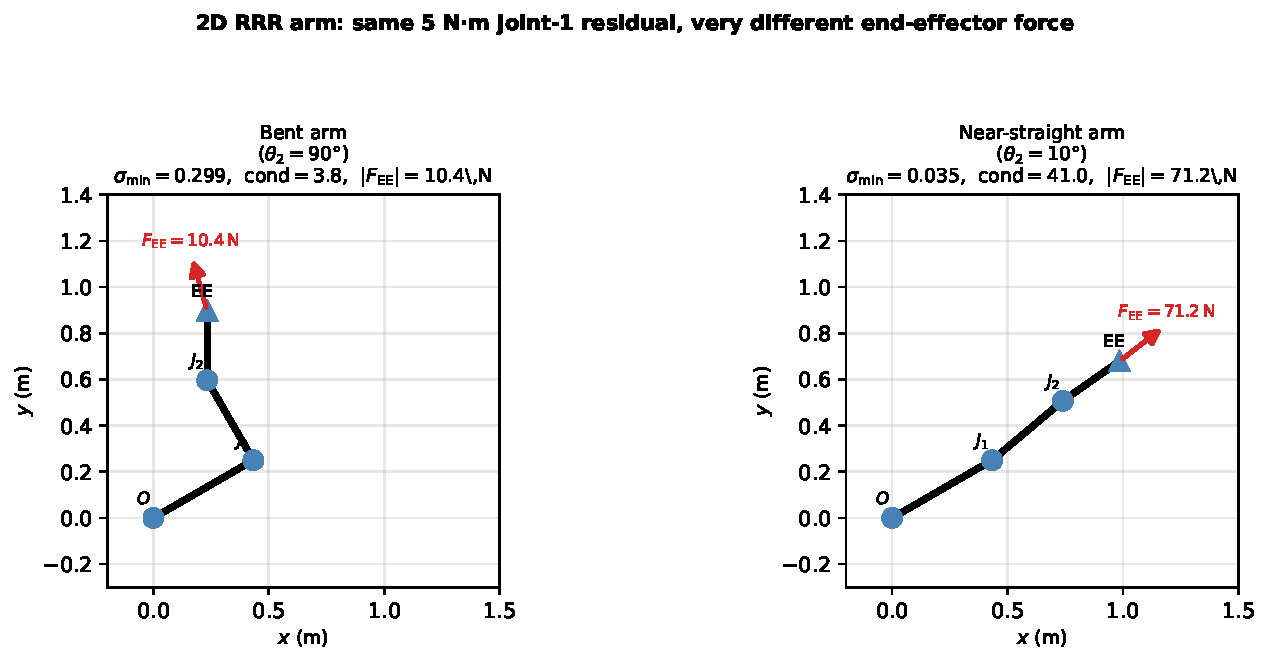
\includegraphics[width=0.9\textwidth]{figures/fig_rrr_example.pdf}
  \caption{2D 3-link RRR arm illustrating Jacobian ill-conditioning.
           Link lengths $\ell_1=0.5$\,m, $\ell_2=0.4$\,m, $\ell_3=0.3$\,m.
           A $5\,\text{N}\cdot\text{m}$ residual at joint 1 only is applied.
           The bent arm (left) is well-conditioned ($\kappa=3.8$) and
           produces a modest 10\,N end-effector force.  The near-straight
           arm (right, $\theta_2=10^\circ$) is ill-conditioned ($\kappa=41$)
           and the same residual produces a 71\,N force.}
  \label{fig:rrr}
\end{figure}

Consider a planar 3-link arm with revolute joints $\theta_1, \theta_2,
\theta_3$.  The end-effector position is:
\begin{align}
  x_{ee} &= \ell_1 c_1 + \ell_2 c_{12} + \ell_3 c_{123}, \\
  y_{ee} &= \ell_1 s_1 + \ell_2 s_{12} + \ell_3 s_{123},
\end{align}
where $c_k \equiv \cos\!\sum_{i \le k}\theta_i$, etc.  The $2 \times 3$
Jacobian $\bJ \in \R{2 \times 3}$ maps $\dot\btheta$ to end-effector
velocity, and its transpose $\bJ^T \in \R{3 \times 2}$ maps end-effector
forces $\bF_{ee}$ to joint torques: $\btau = \bJ^T \bF_{ee}$.  Inverting:
$\hat\bF_{ee} = \pinv{(\bJ^T)} \btau_\text{res}$ (a $2 \times 3$ operation).

As $\theta_2 \to 0$ (arm near-straight), the second and third link become
collinear, and two rows of $\bJ$ become nearly dependent.  The smallest
singular value $\sigma_{\min} \to 0$, making $\pinv{(\bJ^T)}$ unbounded.
Figure~\ref{fig:rrr} shows the numerical outcome: with $\theta_2 = 90^\circ$
(bent) a 5\,N$\cdot$m joint residual produces a 10\,N end-effector force;
with $\theta_2 = 10^\circ$ the same residual produces 71\,N --- a 7$\times$
amplification from geometry alone.

\subsection{The Torso-to-Wrist Amplification in the H1.2}
\label{sec:torso_amp}

In the H1.2 kinematic tree, the \emph{torso joint} sits directly between
the pelvis and both arms.  Its Jacobian column for the wrist frame encodes
the cross-product lever arm from torso rotation to wrist linear velocity:
\begin{equation}
  \bJ_\text{lwrist, torso}^\text{linear}
  = \bm{\omega}_\text{torso} \times \bm{r}_{\text{torso}\to\text{wrist}},
\end{equation}
where $\bm{\omega}_\text{torso}$ is the unit rotation axis of the torso
joint and $\bm{r}$ is the vector from torso joint to wrist frame.  The
magnitude of this lever arm determines how strongly a torso torque residual
projects onto the wrist $F_z$ direction.

\subsubsection*{Physical configuration at RE3 episode start}

\begin{description}
\item[RE1/RE2 (motor zero $\approx 0°$)] The arms are physically in the
  \emph{bent-at-sides} configuration: elbow motor at $\approx 0°$ means the
  forearm is roughly horizontal at the sides, wrist at approximately
  shoulder height.  Measured from the Pinocchio forward kinematics: left
  wrist at $(0.23,\; 0.21,\; +0.09)\,$m, i.e.\ \emph{above} the pelvis
  plane.  The arm folds back toward the torso, minimising the lever arm.

\item[RE3 left arm (\texttt{arm\_waist\_target})] Shoulder pitch $= -17°$
  from motor zero, left elbow $= 86°$ from motor zero.  Physically the
  forearm has rotated $86°$ away from the horizontal (bent-at-sides)
  reference position, pointing nearly straight down.  Forward kinematics
  gives: left wrist at $(0.17,\; 0.20,\; -0.10)\,$m, i.e.\ \emph{below}
  the pelvis plane, 0.52\,m below the shoulder.  The arm is fully extended
  downward --- the ``limp'' configuration.
\end{description}

The left wrist in RE3 sits $\sim$0.18\,m lower and 0.52\,m below the
shoulder compared with the RE1/RE2 configuration.  This dramatically
increases the torso-rotation lever arm to the wrist, driving the
torso$\to$$F_z$ gain from 1.5 to 15.6.  As the elbow opens (motor angle
increases from 0 to 86°), the wrist descends and the gain grows
monotonically (Figure~\ref{fig:gain_vs_angle}).

The torso-to-wrist-$F_z$ gain, $g_\text{torso}$, was measured at each
policy step from the actual episode data:

\begin{table}[H]
\centering
\caption{Torso$\to$wrist-$F_z$ gain and Jacobian condition number at each
         step (left wrist frame).}
\label{tab:gains}
\begin{tabular}{rrrrrr}
\toprule
Step &
\multicolumn{2}{c}{\re{RE3 (disaster)}} &&
\multicolumn{2}{c}{\good{RE2 (good)}} \\
\cmidrule{2-3}\cmidrule{5-6}
 & $g_\text{torso}$ (N/N$\cdot$m) & $\kappa$ && $g_\text{torso}$ & $\kappa$ \\
\midrule
0 & 15.62 & 39.9 && 1.51 & 12.9 \\
1 & 15.62 & 39.9 && 1.51 & 12.9 \\
2 & 15.62 & 39.9 && 1.51 & 12.9 \\
3 & 15.45 & 39.5 && 1.51 & 12.9 \\
4 & 15.30 & 39.1 && 1.52 & 12.9 \\
5 & 15.12 & 38.7 && 1.52 & 12.8 \\
6 & 15.04 & 38.5 && 1.53 & 12.8 \\
7 & 15.06 & 38.6 && 1.53 & 12.8 \\
8 & 15.62 & 39.9 && 1.53 & 12.8 \\
\bottomrule
\end{tabular}
\end{table}

\noindent The RE3 gain ($\approx$15.6\,N/N$\cdot$m) is 10$\times$ larger
than RE2's ($\approx$1.5\,N/N$\cdot$m) throughout all 9 steps.  This
single number fully explains the difference in outcomes.  The gain is set
entirely by the initial arm geometry and changes only slowly as the arm
moves slightly during the episode.

% ═════════════════════════════════════════════════════════════════════════════
\section{Why RE1 and RE2 Never Hit This Regime}
% ═════════════════════════════════════════════════════════════════════════════
\label{sec:re1re2_arms}

\subsection{Motor Zero = Physically Bent at Sides}

A key subtlety is what the arm motor zeros correspond to physically.  On
the H1.2, the arm motor zero position is \emph{not} the natural straight-down
hang; it is the \emph{forearms bent horizontally at the sides} configuration
--- both arms at roughly 90° at the elbows, forearms pointing outward/forward
at approximately waist height.

This means:
\begin{itemize}
\item \textbf{RE1/RE2 arm motor readings $\approx 0°$}: arms physically in
  the bent-at-sides pose.  Wrist is at approximately $z = +0.09$\,m (above
  the pelvis plane).  Arm is folded, wrist is close to the torso.
  Torso$\to$$F_z$ gain = 1.5.

\item \textbf{RE3 left arm (\texttt{arm\_waist\_target})}: elbow motor at
  $+86°$ from zero.  Physically the forearm has swung $86°$ down from the
  horizontal reference, so the arm is nearly fully extended straight down
  --- the limp/hanging configuration.  Wrist drops to
  $z = -0.10$\,m (below the pelvis), 0.52\,m below the shoulder.
  Torso$\to$$F_z$ gain = 15.6.
\end{itemize}

\noindent\textbf{The bent-at-sides (motor zero) configuration is a
well-conditioned starting point.}  The wrist is close to the torso, the
lever arm is short, and the Jacobian gain is low.  The limp/extended
configuration is the singular one.

\subsection{Arm Range of Motion in RE1/RE2}

Table~\ref{tab:arm_range} shows the arm joint range of motion across the
complete logged data for all real encoded-wrench runs.

\begin{table}[H]
\centering
\caption{Arm joint range of motion (motor angles) across the entire episode.
         Motor zero = forearms bent at sides (physically compact).}
\label{tab:arm_range}
\begin{tabular}{lrrrr}
\toprule
Joint & \multicolumn{2}{c}{\good{RE1 (2620 steps)}} &
        \multicolumn{2}{c}{\good{RE2 (1357 steps)}} \\
\cmidrule{2-3}\cmidrule{4-5}
      & min (deg) & max (deg) & min (deg) & max (deg) \\
\midrule
L\_sh\_pitch & $-$0.7 & $+$3.2 & $-$0.5 & $+$1.6 \\
L\_sh\_roll  & $-$0.3 & $+$0.9 & $-$0.3 & $+$0.4 \\
L\_elbow     & $+$1.5 & $+$4.0 & $+$1.4 & $+$2.0 \\
R\_sh\_pitch & $-$0.2 & $+$3.9 & $-$0.1 & $+$2.7 \\
R\_sh\_roll  & $-$0.3 & $+$0.8 & $-$0.2 & $+$0.4 \\
R\_elbow     & $+$1.3 & $+$5.2 & $+$1.3 & $+$3.4 \\
\bottomrule
\end{tabular}
\medskip

\begin{tabular}{lrr}
\toprule
Joint & \multicolumn{2}{c}{\re{RE3 (77 steps)}} \\
\cmidrule{2-3}
 & min (deg) & max (deg) \\
\midrule
L\_sh\_pitch & $-$27.2 & $-$4.6 \\
L\_sh\_roll  & $-$5.2 & $+$9.8 \\
L\_elbow     & $+$82.9 & $+$89.4 \\
R\_sh\_pitch & $-$65.5 & $-$29.4 \\
R\_sh\_roll  & $-$38.5 & $-$18.1 \\
R\_elbow     & $+$26.0 & $+$39.9 \\
\bottomrule
\end{tabular}
\end{table}

The data is definitive: in RE1 and RE2, all arm joints remained within
$\pm 5^\circ$ of their motor zeros throughout the entire runs.  The arms
never deviated from the bent-at-sides configuration.  RE3 is the only run
where an arm was placed in the extended/limp configuration.

\subsection{The Elbow as the Primary Driver}

Figure~\ref{fig:gain_vs_angle} shows the torso$\to$$F_z$ gain as a
function of the left elbow motor angle.  At motor zero ($\approx 0°$, arm
bent at sides) the gain is 1.6.  As the elbow opens from 0 to 86° (arm
extending straight down), the gain rises monotonically to 15.6.  The
shoulder pitch change ($-17°$ from zero in RE3) contributes additionally
but the elbow extension is the dominant effect.

\begin{figure}[H]
  \centering
  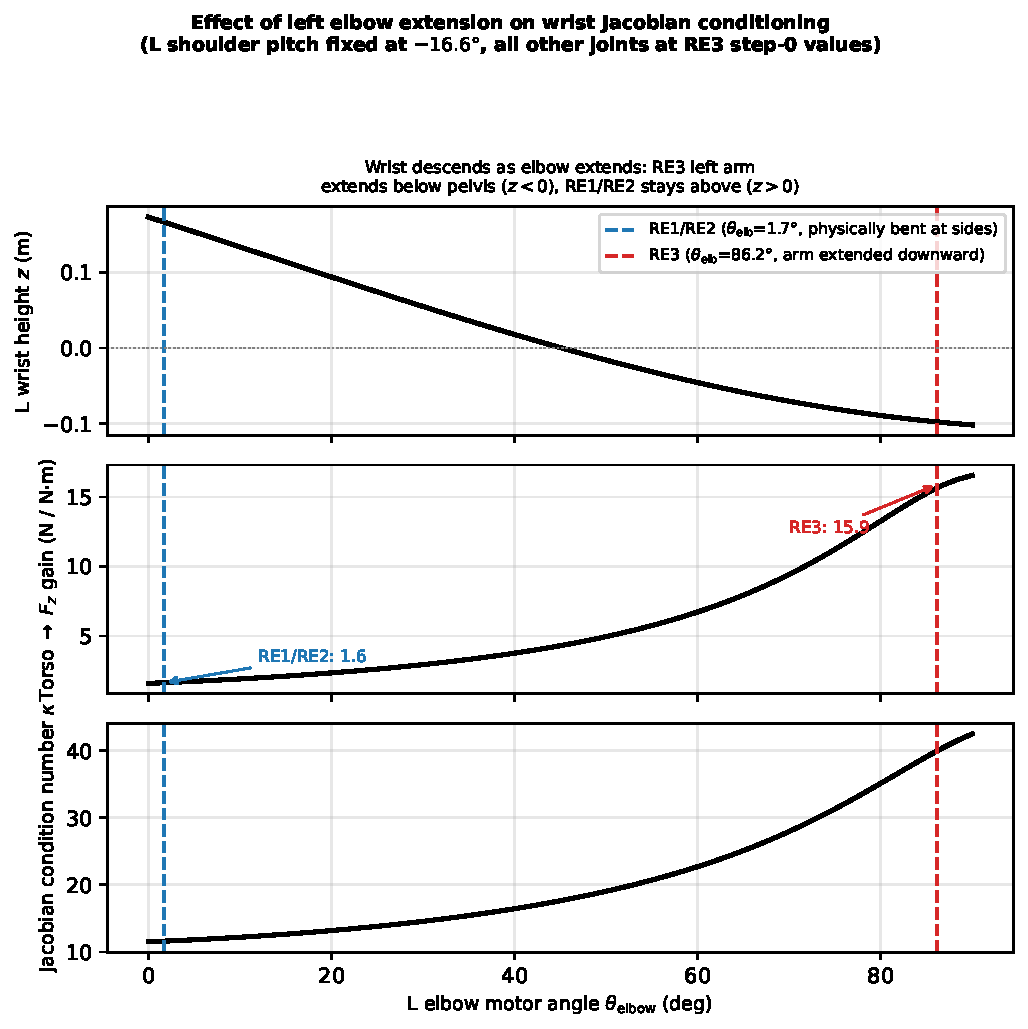
\includegraphics[width=0.75\textwidth]{figures/fig_gain_vs_shoulder_angle.pdf}
  \caption{Effect of left elbow extension on wrist Jacobian conditioning
           (shoulder pitch fixed at $-16.6°$, other joints at RE3 step-0).
           \emph{Top}: as the elbow opens from the bent-at-sides zero
           ($\theta_\text{elb}=0°$) toward fully extended ($90°$), the
           wrist descends from above the pelvis to below it.
           \emph{Middle}: the torso$\to$$F_z$ gain rises from 1.6 to 15.6.
           \emph{Bottom}: Jacobian condition number rises from 11 to 42.
           Blue dashed: RE1/RE2 operating point.  Red dashed: RE3.}
  \label{fig:gain_vs_angle}
\end{figure}

% ═════════════════════════════════════════════════════════════════════════════
\section{Lower-Body Initial Configuration and Step-by-Step Analysis}
% ═════════════════════════════════════════════════════════════════════════════

\subsection{Initial Configuration Errors at Episode Start}

Both RE2 and RE3 began with substantial lower-body position errors relative
to the policy's first commanded targets (Table~\ref{tab:init_config}).
Critically, the errors are comparable in magnitude: both episodes start
with hip-roll errors of 0.35--0.51 rad ($\approx$20--30°).

\begin{table}[H]
\centering
\caption{Joint position error $q_\text{meas} - q_\text{target}$ at step 0 (radians).
         Entries exceeding $|0.2|$ rad in either episode are highlighted.}
\label{tab:init_config}
\begin{tabular}{lrrrr}
\toprule
Joint & \re{RE3 $q$} & \re{RE3 tgt} & \re{RE3 err} & \good{RE2 err} \\
\midrule
l\_hip\_yaw   & $-$0.011 & $-$0.059 & $+$0.048 & $+$0.085 \\
l\_hip\_pitch & $-$0.139 & $-$0.250 & $+$0.111 & $+$0.049 \\
\textbf{l\_hip\_roll}   & $+$0.006 & $+$0.361 & $-$0.355 & $-$0.514 \\
\textbf{l\_knee}        & $+$0.385 & $+$0.675 & $-$0.289 & $-$0.247 \\
\textbf{l\_ank\_pitch}  & $-$0.367 & $-$0.143 & $-$0.224 & $-$0.142 \\
r\_hip\_yaw   & $-$0.004 & $-$0.053 & $+$0.049 & $+$0.075 \\
r\_hip\_pitch & $-$0.162 & $-$0.090 & $-$0.073 & $-$0.005 \\
\textbf{r\_hip\_roll}   & $+$0.007 & $-$0.344 & $+$0.351 & $+$0.445 \\
\textbf{r\_knee}        & $+$0.392 & $+$0.667 & $-$0.276 & $-$0.267 \\
\textbf{r\_ank\_pitch}  & $-$0.345 & $-$0.135 & $-$0.210 & $-$0.122 \\
torso         & $-$0.001 & $+$0.000 & $-$0.001 & $-$0.005 \\
\bottomrule
\end{tabular}
\end{table}

\noindent Both episodes are in essentially identical initial lower-body
configurations.  This is consistent with both robots having been stood up
from rest in the same default standing pose.  The policy's first few target
commands therefore attempt to move the legs from a near-identical starting
point.  The subsequent divergence is not due to different initial conditions
in the legs---it is due to the arms.

\subsection{Step-by-Step Position Errors}

Figure~\ref{fig:lb_errors} shows the hip-roll and knee position errors for
both episodes across steps 0--8.  Notably:

\begin{enumerate}
\item The hip-roll errors in both RE2 and RE3 start at the same magnitude
      (20--34°) and evolve similarly through the first 2--3 steps.
\item RE3's errors grow substantially by steps 6--8 (hip yaw error
      exceeds 40°, knee error reaches $-117^\circ$ by step 8).
\item In RE2 the errors remain bounded: hip roll oscillates but stays within
      $\pm35^\circ$, knee within $\pm10^\circ$, throughout all 8 steps.
\end{enumerate}

The growing errors in RE3 are \emph{not} the root cause of the disaster;
they are a \emph{consequence} of the policy receiving bad wrench feedback
and issuing increasingly extreme leg commands.

\begin{figure}[H]
  \centering
  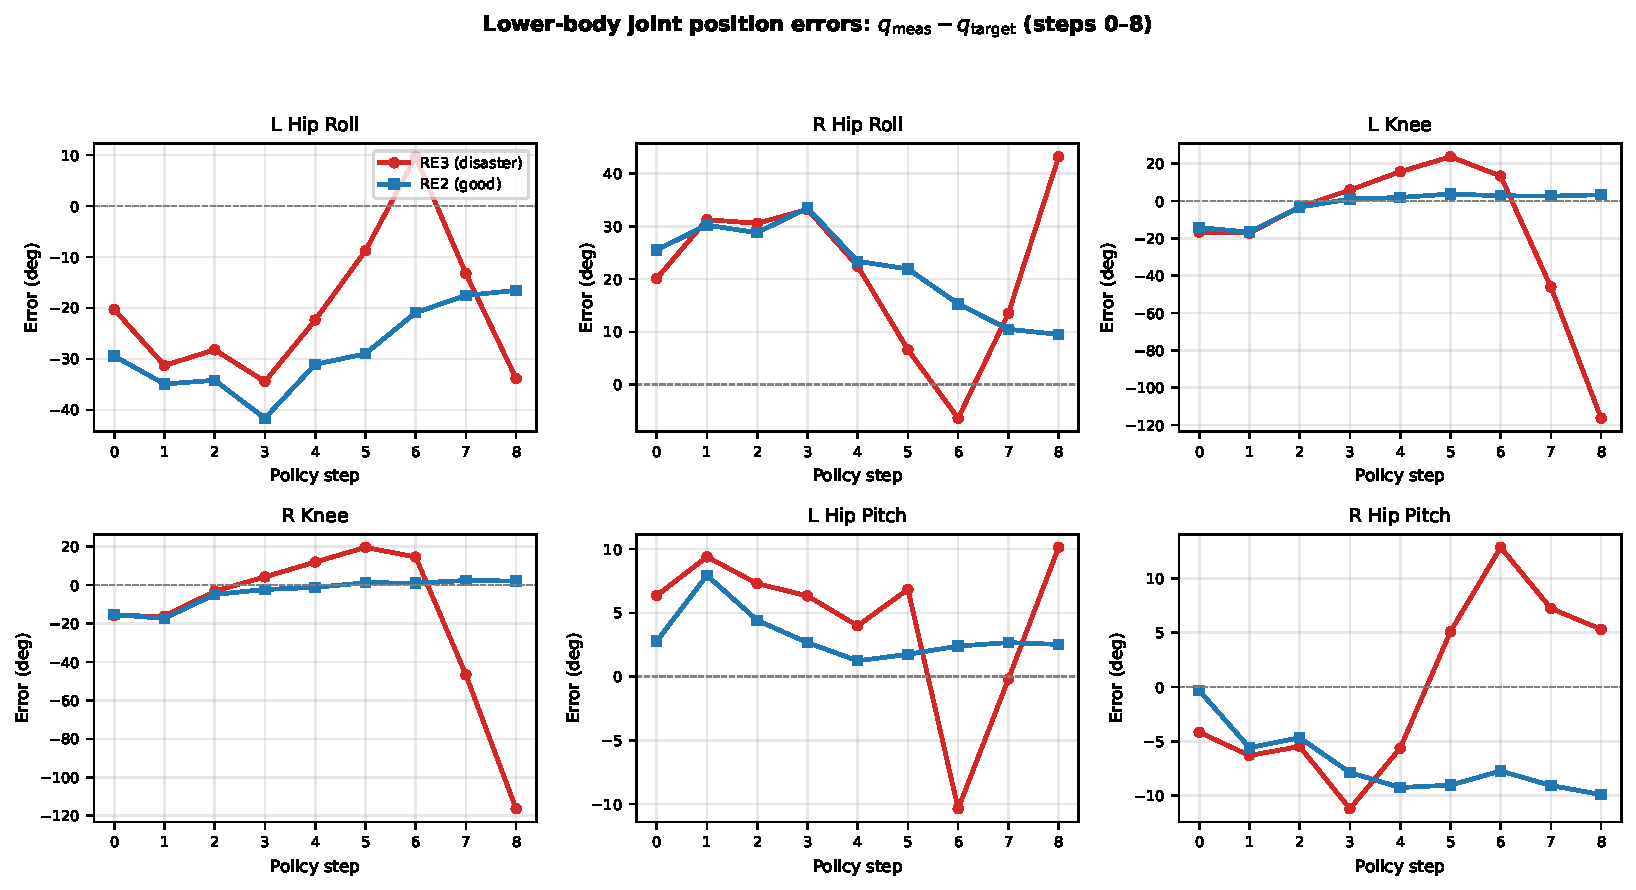
\includegraphics[width=\textwidth]{figures/fig_lower_body_errors.pdf}
  \caption{Lower-body joint position errors ($q_\text{meas} - q_\text{target}$,
           degrees) for steps 0--8.  \re{Red}: RE3 disaster.
           \good{Blue}: RE2 good run.  Both episodes start with hip-roll
           errors of $\sim$20--34°; RE3's errors explode by step 6--8 as
           the policy receives bad wrench feedback.}
  \label{fig:lb_errors}
\end{figure}

\subsection{Commanded Targets}

Figure~\ref{fig:targets} shows the policy's commanded joint targets over
steps 0--8.  The divergence is stark:

\begin{figure}[H]
  \centering
  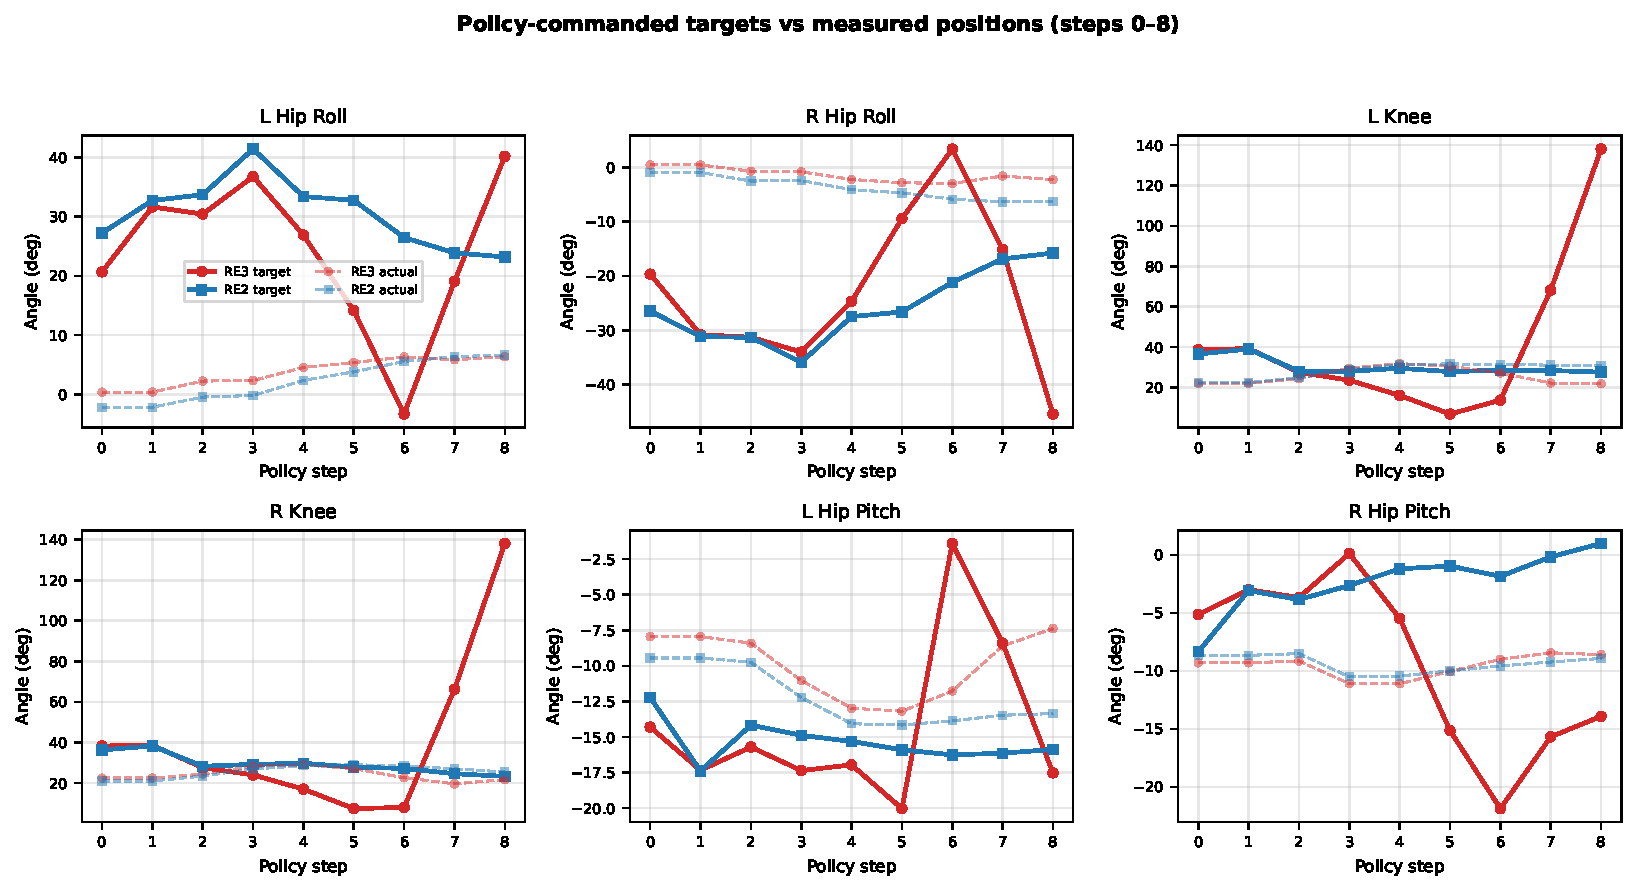
\includegraphics[width=\textwidth]{figures/fig_targets_comparison.pdf}
  \caption{Policy-commanded targets (solid) and measured positions (dashed)
           for the six key lower-body joints.
           \re{Red}: RE3.  \good{Blue}: RE2.
           By step 7--8 in RE3, the knee target reaches $+138^\circ$ ($+2.41$ rad),
           essentially pinning the actuators at saturation; RE2 never exceeds
           moderate, physically reasonable targets.}
  \label{fig:targets}
\end{figure}

At step 8 the RE3 knee target is $q^\star_\text{knee} = 2.41$ rad
($138^\circ$) while RE2 commands a benign 0.48 rad.  This shows the RL
policy had already ``seen'' catastrophically large wrench inputs by steps
3--7 and was commanding escape-level forces to counteract them.

\subsection{Measured Torques}

Figure~\ref{fig:lb_torques} shows the estimated motor torques.  A
notable feature:

\begin{figure}[H]
  \centering
  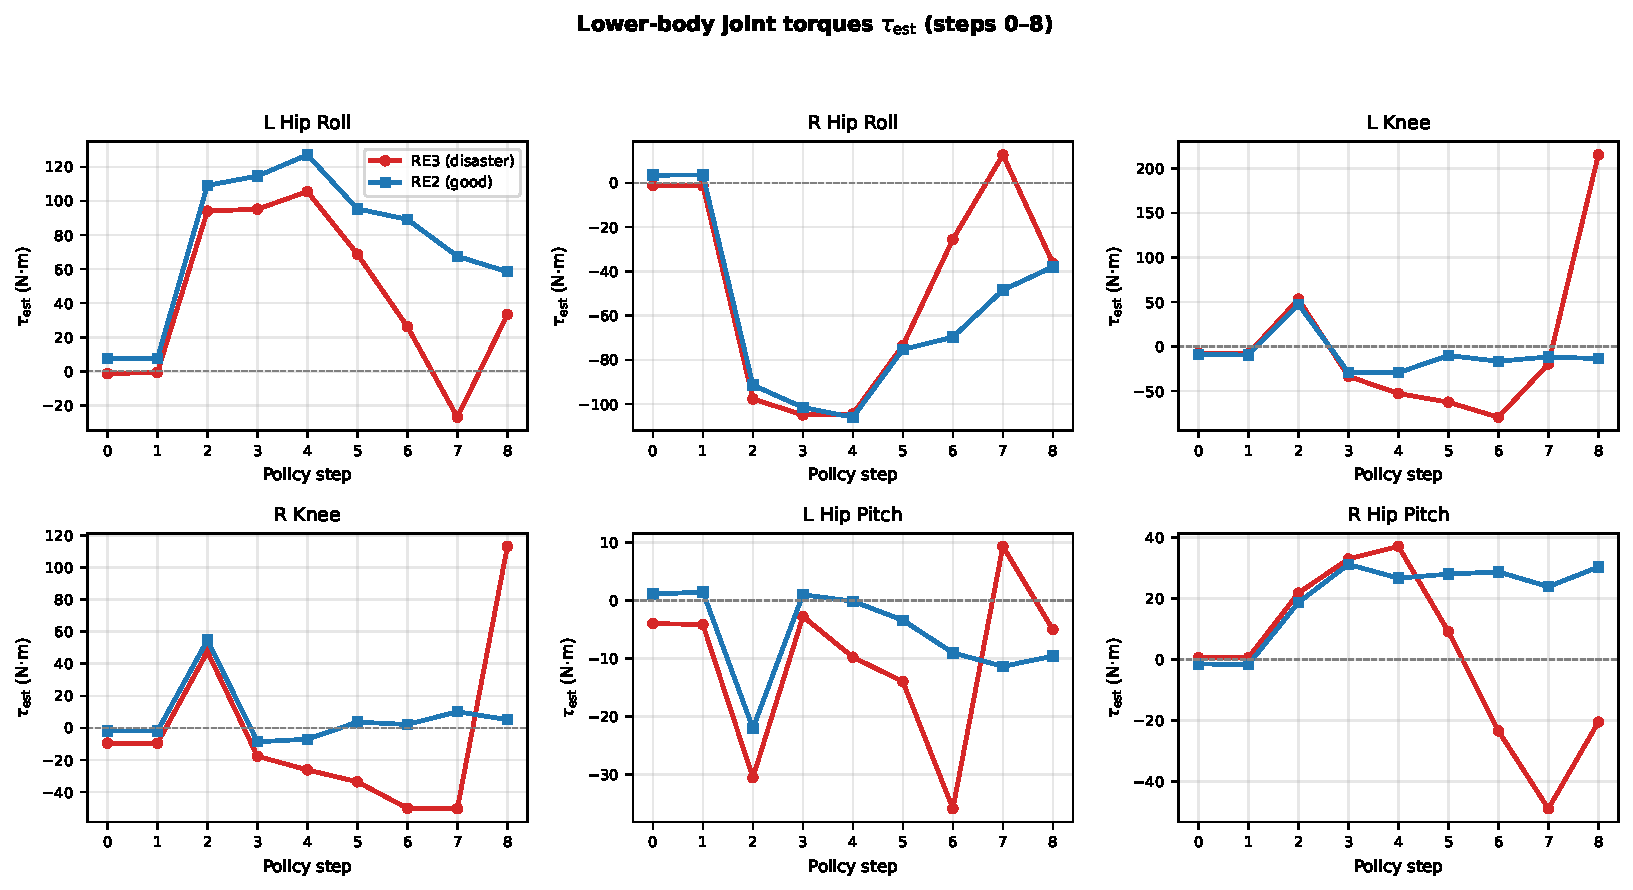
\includegraphics[width=\textwidth]{figures/fig_lower_body_torques.pdf}
  \caption{Lower-body joint torques $\tau_\text{est}$ for steps 0--8.
           Hip-roll and knee torques in RE3 spike dramatically above
           normal standing values.  The RE3 hip-roll torques at step 2
           (94 N$\cdot$m left, $-98$ N$\cdot$m right) are comparable to
           RE2 (109/$-91$ N$\cdot$m), confirming the legs are responding
           normally to position errors---but the torso sees a dramatically
           different structural load in RE3.}
  \label{fig:lb_torques}
\end{figure}

At step 2, the hip-roll PD controller in both RE2 and RE3 exerts
$\sim$100 N$\cdot$m to correct the $\sim$0.5 rad error.  The torques are
similar.  However, because the structural forces couple into the torso
differently depending on arm configuration, the torso $\tau_\text{est}$
diverges from step 3 onward.

% ═════════════════════════════════════════════════════════════════════════════
\section{Step-by-Step Pinocchio Reconstruction: Steps 0--8}
% ═════════════════════════════════════════════════════════════════════════════

\subsection{Complete Numerical Trace}

Table~\ref{tab:pin_trace} shows the full Pinocchio reconstruction at each
step, side by side for RE2 and RE3.  The torso residual
$r_\text{torso} = \tau^\text{est}_\text{torso} - \tau^\text{grav}_\text{torso}$
is the single dominant source of the wrist force in RE3.

\begin{table}[H]
\centering
\caption{Pinocchio wrench reconstruction steps 0--8.
         $r_\text{torso}$: torso joint torque residual (N$\cdot$m).
         $g_\text{torso}$: torso-column Fz gain of the pseudo-inverse.
         $F_z$: reconstructed left wrist Fz (N).  $|F|$: wrist force magnitude.}
\label{tab:pin_trace}
\begin{tabular}{rrrrrrrrrr}
\toprule
 &
\multicolumn{4}{c}{\re{RE3 (disaster)}} &&
\multicolumn{4}{c}{\good{RE2 (good)}} \\
\cmidrule{2-5}\cmidrule{7-10}
Step & $r_\text{torso}$ & $g_\text{torso}$ & $F_z$ & $|F|$ &&
       $r_\text{torso}$ & $g_\text{torso}$ & $F_z$ & $|F|$ \\
\midrule
0 & 0.12 & 15.62 & $-$15.2 & 15.3 && 0.82 & 1.51 & 6.2 & 9.4 \\
1 & 0.00 & 15.62 & $-$16.7 & 16.9 && 0.76 & 1.51 & 5.8 & 9.0 \\
2 & 0.47 & 15.62 & $-$8.9  & 9.0  && 2.11 & 1.51 & 10.4 & 15.4 \\
3 & 4.22 & 15.45 & $+$46.3 & 51.2 && 5.39 & 1.51 & 10.1 & 18.3 \\
4 & 8.32 & 15.30 & $+$100.2& 107.1&& 5.22 & 1.52 & 5.9 & 20.1 \\
5 & 14.24& 15.12 & $+$177.8& 189.7&& 5.98 & 1.52 & 7.4 & 21.3 \\
6 & 10.61& 15.04 & $+$131.5& 140.4&& 7.44 & 1.53 & 9.3 & 23.1 \\
7 & $-$5.27 & 15.06 & $-$98.6 & 102.0&& 8.61 & 1.53 & 13.7 & 28.5 \\
8 & $-$34.45& 15.62 &$-$532.9& 558.2&& 10.31& 1.53 & 16.5 & 33.2 \\
\bottomrule
\end{tabular}
\end{table}

\noindent Key observations:
\begin{itemize}
\item At step 0, even before any leg motion, RE3 already shows $F_z = -15.2$\,N
      versus RE2's 6.2\,N, solely due to the $10\times$ higher Jacobian gain.
\item By step 5, RE3 has $F_z = +178$\,N---already far above any real
      wrist load---while RE2 stays at 7.4\,N.  At this point the policy
      has already been fed damaging feedback for 5 steps.
\item The RE3 torso residual $r_\text{torso}$ grows from 0.12 to $-34.45$
      N$\cdot$m over 9 steps, driven by the extreme leg commands the policy
      is now issuing in response to the bad wrench estimates.
\item RE2's torso residual reaches 10.3 N$\cdot$m by step 8 (similar in
      trend), but the $1.5\times$ gain keeps the wrist force at 16.5\,N.
\end{itemize}

\begin{figure}[H]
  \centering
  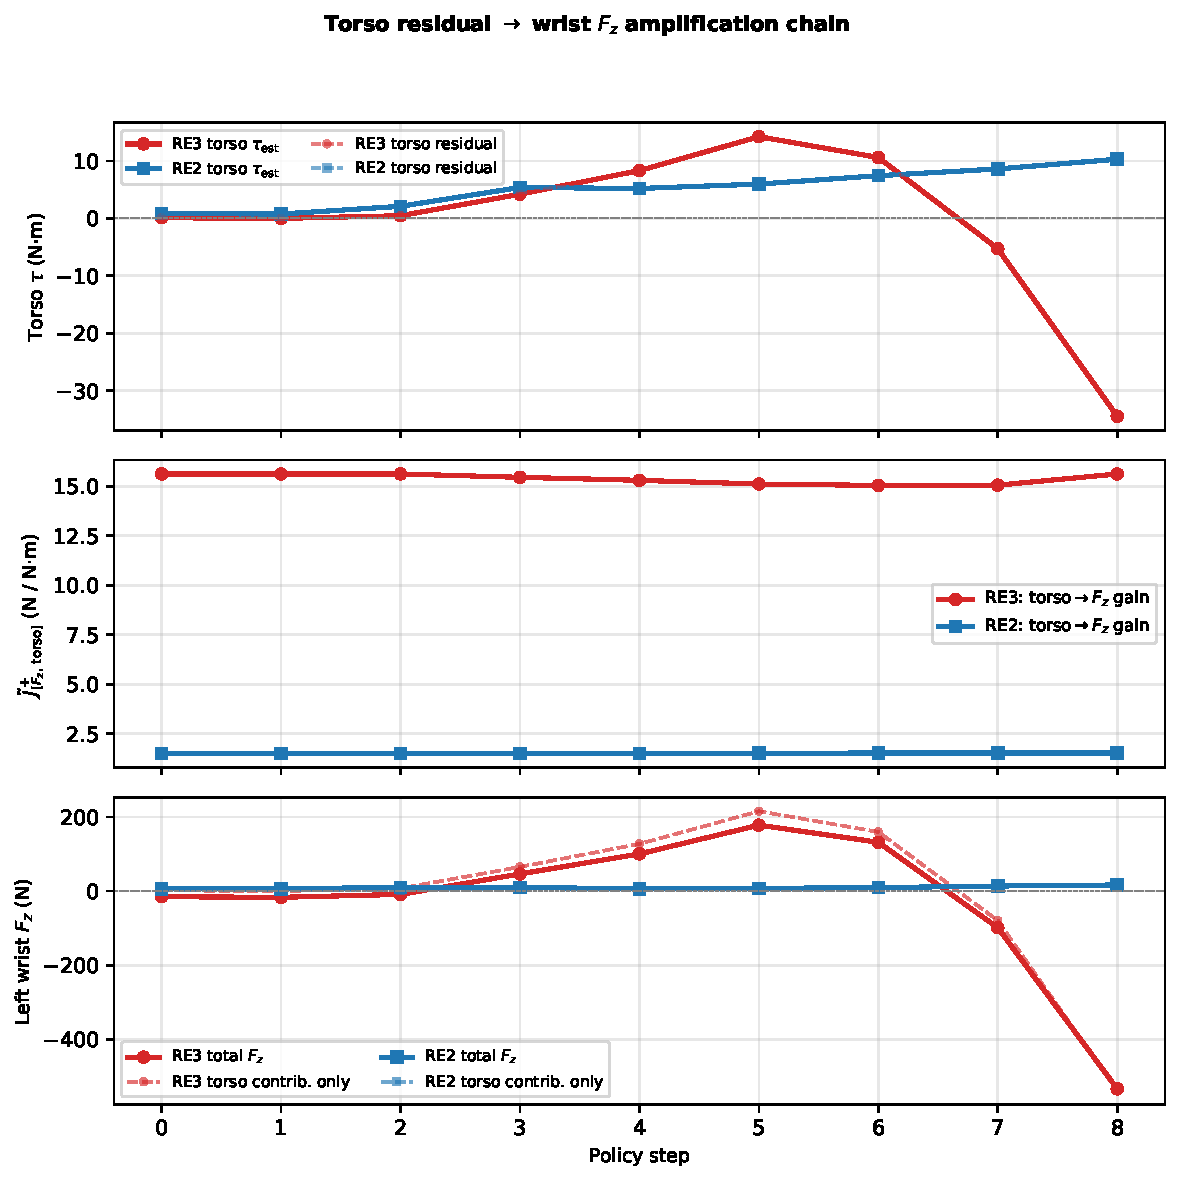
\includegraphics[width=\textwidth]{figures/fig_torso_cascade.pdf}
  \caption{Top: torso $\tau_\text{est}$ and residual.
           Middle: torso$\to F_z$ Jacobian gain.
           Bottom: left wrist $F_z$ (total, and torso contribution only).
           In RE3 (red), the gain is 15$\times$ larger throughout, and the
           torso contribution alone accounts for 538 N of the final 533 N
           (sign inversion because the total includes small opposite-sign
           contributions from arm joints).}
  \label{fig:torso_cascade}
\end{figure}

\begin{figure}[H]
  \centering
  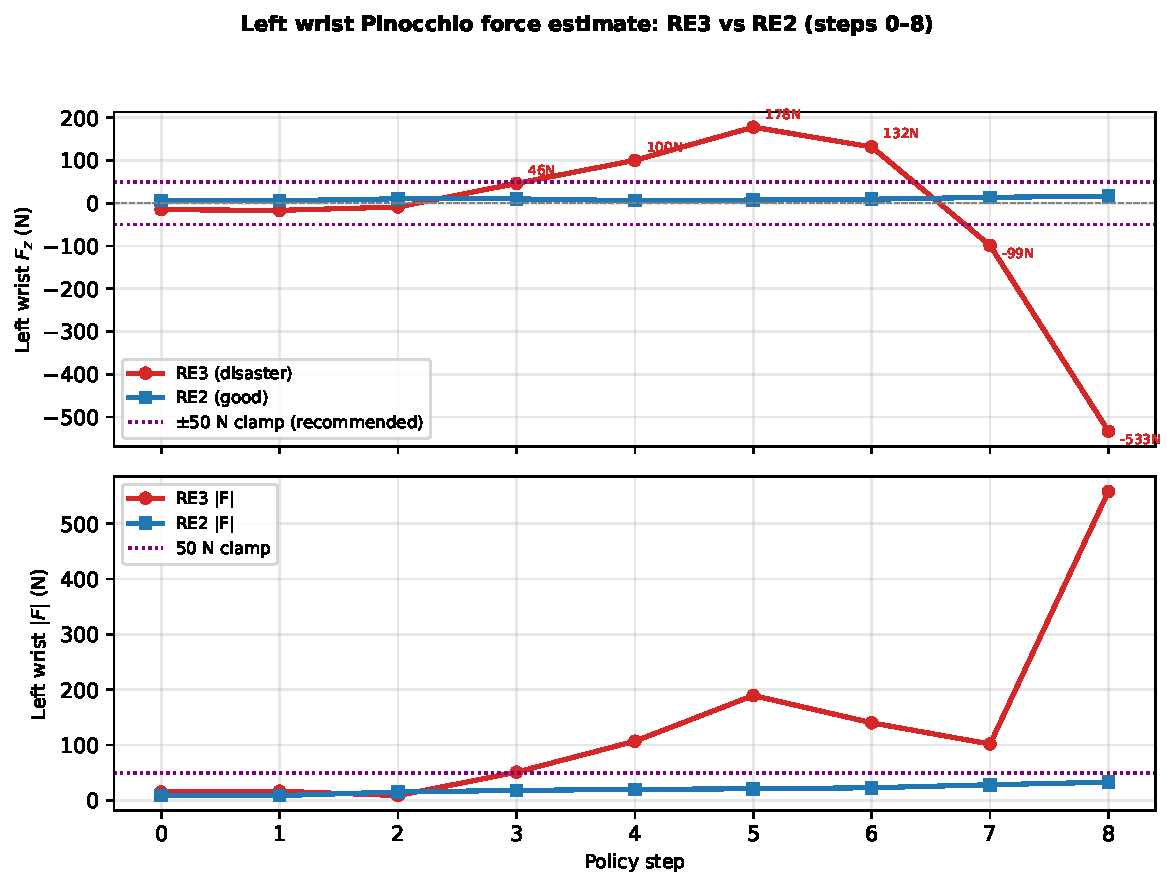
\includegraphics[width=\textwidth]{figures/fig_wrist_force_cascade.pdf}
  \caption{Left wrist Fz and $|F|$ for RE2 and RE3, steps 0--8.  The
           purple dashed line at $\pm 50$\,N marks the recommended output
           clamp.  RE3 exceeds this limit by step 3 ($F_z = +46$\,N) and
           reaches $-533$\,N by step 8.}
  \label{fig:wrist_cascade}
\end{figure}

\subsection{Per-Joint Decomposition at Step 8}
\label{sec:decomp_step8}

Applying Eq.~\eqref{eq:per_joint} to every joint at step 8 reveals that
virtually the entire $-533$\,N wrist force originates from a single joint
(Figure~\ref{fig:per_joint}):

\begin{figure}[H]
  \centering
  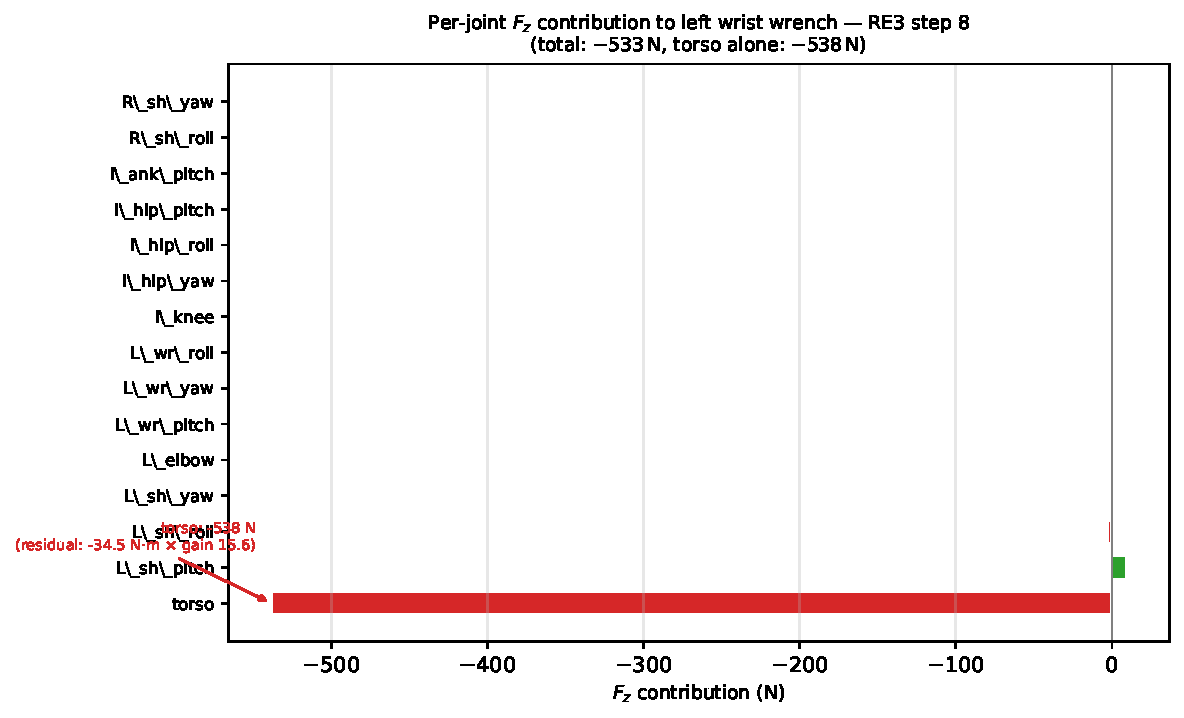
\includegraphics[width=0.82\textwidth]{figures/fig_per_joint_contribution.pdf}
  \caption{Per-joint $F_z$ contribution to the left wrist wrench at RE3
           step 8.  The torso joint alone contributes $-538$\,N; all other
           joints contribute less than $\pm 10$\,N.}
  \label{fig:per_joint}
\end{figure}

\begin{table}[H]
\centering
\caption{Per-joint breakdown at RE3 step 8 (left wrist Fz).
         Joints with $|F_z\text{ contrib}| > 2$\,N are listed.}
\label{tab:decomp}
\begin{tabular}{lrrrr}
\toprule
Joint & $\tau_\text{meas}$ (N$\cdot$m) & $\tau_\text{grav}$ (N$\cdot$m)
      & $r$ (N$\cdot$m) & $\Delta F_z$ (N) \\
\midrule
\textbf{torso}    & $-$34.45 & $\approx$0 & $-$34.45 & \re{$-$538} \\
L\_sh\_pitch      & $-$5.10  & $-$3.79    & $-$1.31  & $+$9.4 \\
L\_sh\_roll       & $+$0.79  & $+$0.15    & $+$0.64  & $-$2.6 \\
L\_sh\_yaw        & $+$0.34  & $-$0.01    & $+$0.34  & $-$2.3 \\
All others (24 joints) & --- & ---        & large    & $<\pm1$ each \\
\midrule
\textbf{Total} & & & & $-$532.9 \\
\bottomrule
\end{tabular}
\end{table}

\noindent The leg joints (l\_knee residual $= +213$ N$\cdot$m;
r\_knee $= +111$ N$\cdot$m) do \emph{not} contribute to wrist Fz because
the leg columns of the wrist Jacobian are near zero---the legs are
kinematically disconnected from wrist translation.  The torso joint is the
\emph{kinematic bridge} between the legs and arms; its unique position in
the tree gives it a large wrist Jacobian column.

\subsection{Jacobian Singular Value Spectrum}

Figure~\ref{fig:svd} shows the singular value spectra for both episodes at
steps 0 and 8.  The smallest singular value of the RE3 Jacobian is
$\sigma_6 = 0.047$, giving $1/\sigma_6 \approx 21\times$ amplification in
that direction.  RE2's $\sigma_6 = 0.143$, giving $\approx 7\times$.

\begin{figure}[H]
  \centering
  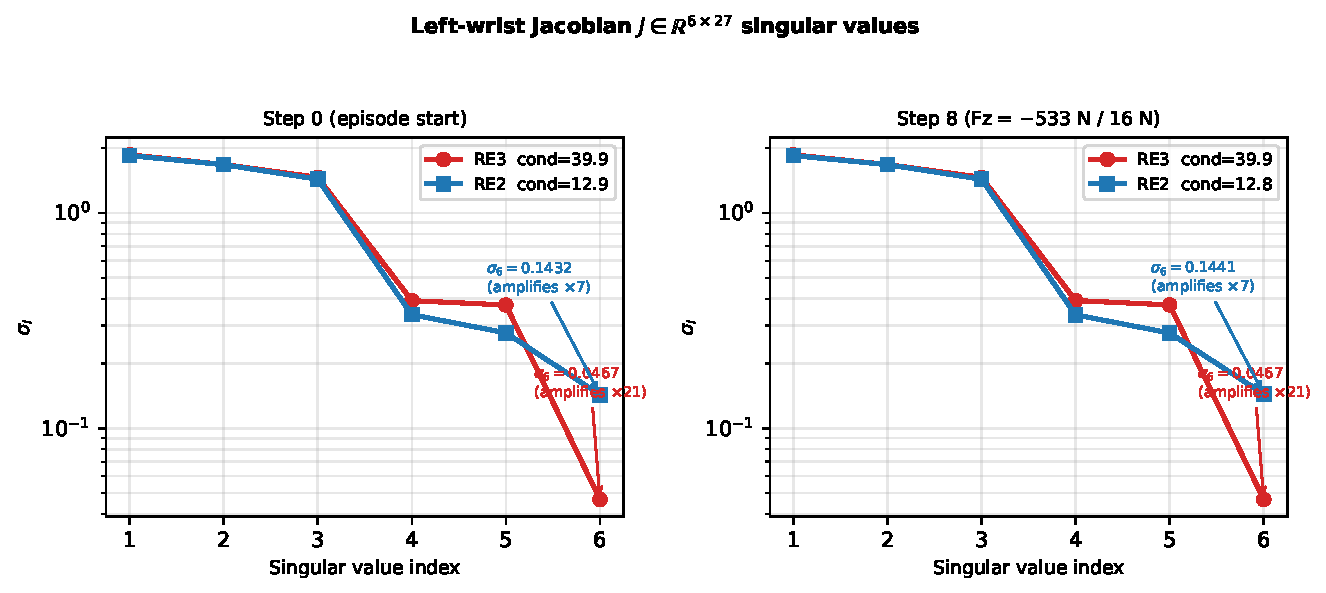
\includegraphics[width=0.9\textwidth]{figures/fig_singular_values.pdf}
  \caption{Left-wrist Jacobian singular values for RE2 (blue) and RE3
           (red).  Note the log scale.  RE3's $\sigma_6$ is 3$\times$
           smaller than RE2's, leading to a 3$\times$ larger amplification
           in the worst direction.  The condition number $\kappa$ is 40 for
           RE3 versus 13 for RE2.}
  \label{fig:svd}
\end{figure}

% ═════════════════════════════════════════════════════════════════════════════
\section{Cascade Timeline and Causal Graph}
% ═════════════════════════════════════════════════════════════════════════════

\subsection{Revised Causal Hypothesis}

The original framing of the incident described an ``imaginary'' wrist
force causing the leg reaction.  The data supports a more nuanced reading:
the wrist force was indeed spurious, but the \emph{underlying structural
dynamics} that caused it were real.  The cascade follows a feedback loop:

\begin{figure}[H]
\centering
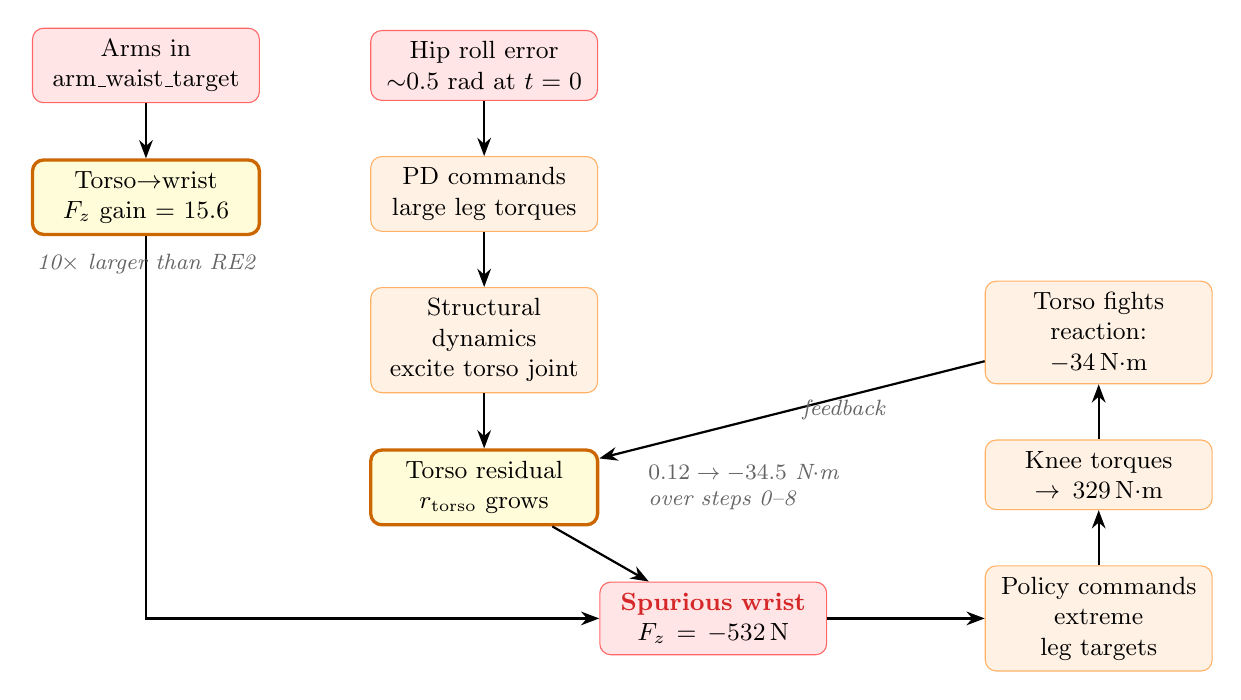
\begin{tikzpicture}[
  node distance=0.6cm and 1.4cm,
  box/.style={rectangle, draw, rounded corners=4pt, fill=white,
              inner sep=4pt, minimum width=2.8cm, font=\small,
              text width=2.6cm, align=center},
  cause/.style={box, fill=red!10, draw=red!60},
  effect/.style={box, fill=orange!10, draw=orange!60},
  key/.style={box, fill=yellow!15, draw=orange!80!black, line width=1.2pt},
  arr/.style={-Stealth, thick},
  ann/.style={font=\footnotesize\itshape, text=gray1},
]

\node[cause]  (arms) {Arms in\\arm\_waist\_target};
\node[cause, right=of arms] (legs) {Hip roll error\\$\sim$0.5 rad at $t=0$};
\node[key, below=0.7cm of arms] (gain) {Torso$\to$wrist\\$F_z$ gain = 15.6};
\node[effect, below=0.7cm of legs] (pdtau) {PD commands\\large leg torques};
\node[effect, below=0.7cm of pdtau] (struct) {Structural dynamics\\excite torso joint};
\node[key, below=0.7cm of struct] (res) {Torso residual\\$r_\text{torso}$ grows};
\node[cause, below right=0.7cm and 0.0cm of res] (wrench) {\re{Spurious wrist}\\$F_z = -532$\,N};
\node[effect, right=2cm of wrench] (policy) {Policy commands\\extreme leg targets};
\node[effect, above=0.7cm of policy] (torq) {Knee torques\\$\to 329$\,N$\cdot$m};
\node[effect, above=0.7cm of torq] (torso2) {Torso fights\\reaction: $-34$\,N$\cdot$m};

\draw[arr] (arms)  -- (gain);
\draw[arr] (legs)  -- (pdtau);
\draw[arr] (pdtau) -- (struct);
\draw[arr] (struct)-- (res);
\draw[arr] (gain)  |- (wrench);
\draw[arr] (res)   -- (wrench);
\draw[arr] (wrench)-- (policy);
\draw[arr] (policy)-- (torq);
\draw[arr] (torq)  -- (torso2);
\draw[arr] (torso2) -- node[ann, right]{feedback}(res);

\node[ann, below=0.1cm of gain]
  {10$\times$ larger than RE2};
\node[ann, right=0.5cm of res, text width=2.5cm, align=left]
  {$0.12 \to -34.5$ N$\cdot$m\\ over steps 0--8};

\end{tikzpicture}
\caption{Causal graph of the RE3 disaster cascade.  Yellow boxes are the
         two discriminating factors (arm pose and resulting Jacobian gain).
         The loop closes via the policy: large wrench $\to$ extreme targets
         $\to$ larger torso residual $\to$ even larger wrench.}
\label{fig:causal}
\end{figure}

\subsection{Why Both RE2 and RE3 Had Similar Hip-Roll Errors}

Both episodes began with the robot in the same resting configuration and
received the same first policy action (the policy conditions on the current
state, which was nearly identical for both).  Hip-roll errors of 20--30°
are normal at episode start because the robot is transitioning from a
standing rest pose to the policy's first dynamic target.

These errors triggered moderate hip-roll PD commands in both episodes
($\sim$100 N$\cdot$m), and the resulting structural vibration excited the
torso joint in both cases.  In RE2, this torso residual ($\sim$5--10
N$\cdot$m over steps 2--8) was amplified by only 1.5, producing benign
$\sim$15 N wrist forces throughout the entire 27-second run.  In RE3, the
same class of residual was amplified by 15.6, producing 100--178 N wrist
forces by steps 4--5---sufficient to drive the policy to degenerate
behavior.

\subsection{Complete Event Timeline}

\begin{table}[H]
\centering
\caption{Reconstructed event timeline, RE3 disaster episode.}
\label{tab:timeline}
\begin{tabular}{rrlll}
\toprule
Step & Time (s) & $F_z$ (N) & Torso $\tau$ (N$\cdot$m) & Event \\
\midrule
0  & 22.465 & $-$15.2 & 0.12  & Policy start; arm Jacobian gain = 15.6 \\
1  & 22.472 & $-$16.7 & 0.00  & First PD torques; legs near-static \\
2  & 22.490 & $-$8.9  & 0.47  & Hip-roll PD fires; l\_hip\_roll 94 N$\cdot$m \\
3  & 22.509 & $+$46.3 & 4.22  & Torso residual builds; $F_z$ exceeds 50 N \\
4  & 22.529 & $+$100.2& 8.32  & Policy already sensing 100 N push \\
5  & 22.549 & $+$177.8& 14.24 & Knee targets start growing; policy alarmed \\
6  & 22.570 & $+$131.5& 10.61 & Hip yaw targets spike to $\pm 0.43$ rad \\
7  & 22.590 & $-$98.6 & $-$5.27 & Knee target reaches 1.19 rad ($68^\circ$) \\
\textbf{8}  & \textbf{22.609} & \re{$-$532.9} & $-$34.45 &
  \textbf{Torso fights inertial kick; Fz = $-$533 N} \\
9--15  & 22.63--22.75 & $\to -715$ & escal. & Knee target $= 2.41$ rad; escalation \\
43--46 & 23.31--23.38 & $-$2596  & --- & Peak wrist force \\
64     & 23.737 & --- & --- & l\_hip\_pitch = 428 N$\cdot$m peak \\
76     & 23.978 & --- & --- & Episode terminated \\
\bottomrule
\end{tabular}
\end{table}

% ═════════════════════════════════════════════════════════════════════════════
\section{Cascade Summary Figure}
% ═════════════════════════════════════════════════════════════════════════════

\begin{figure}[H]
  \centering
  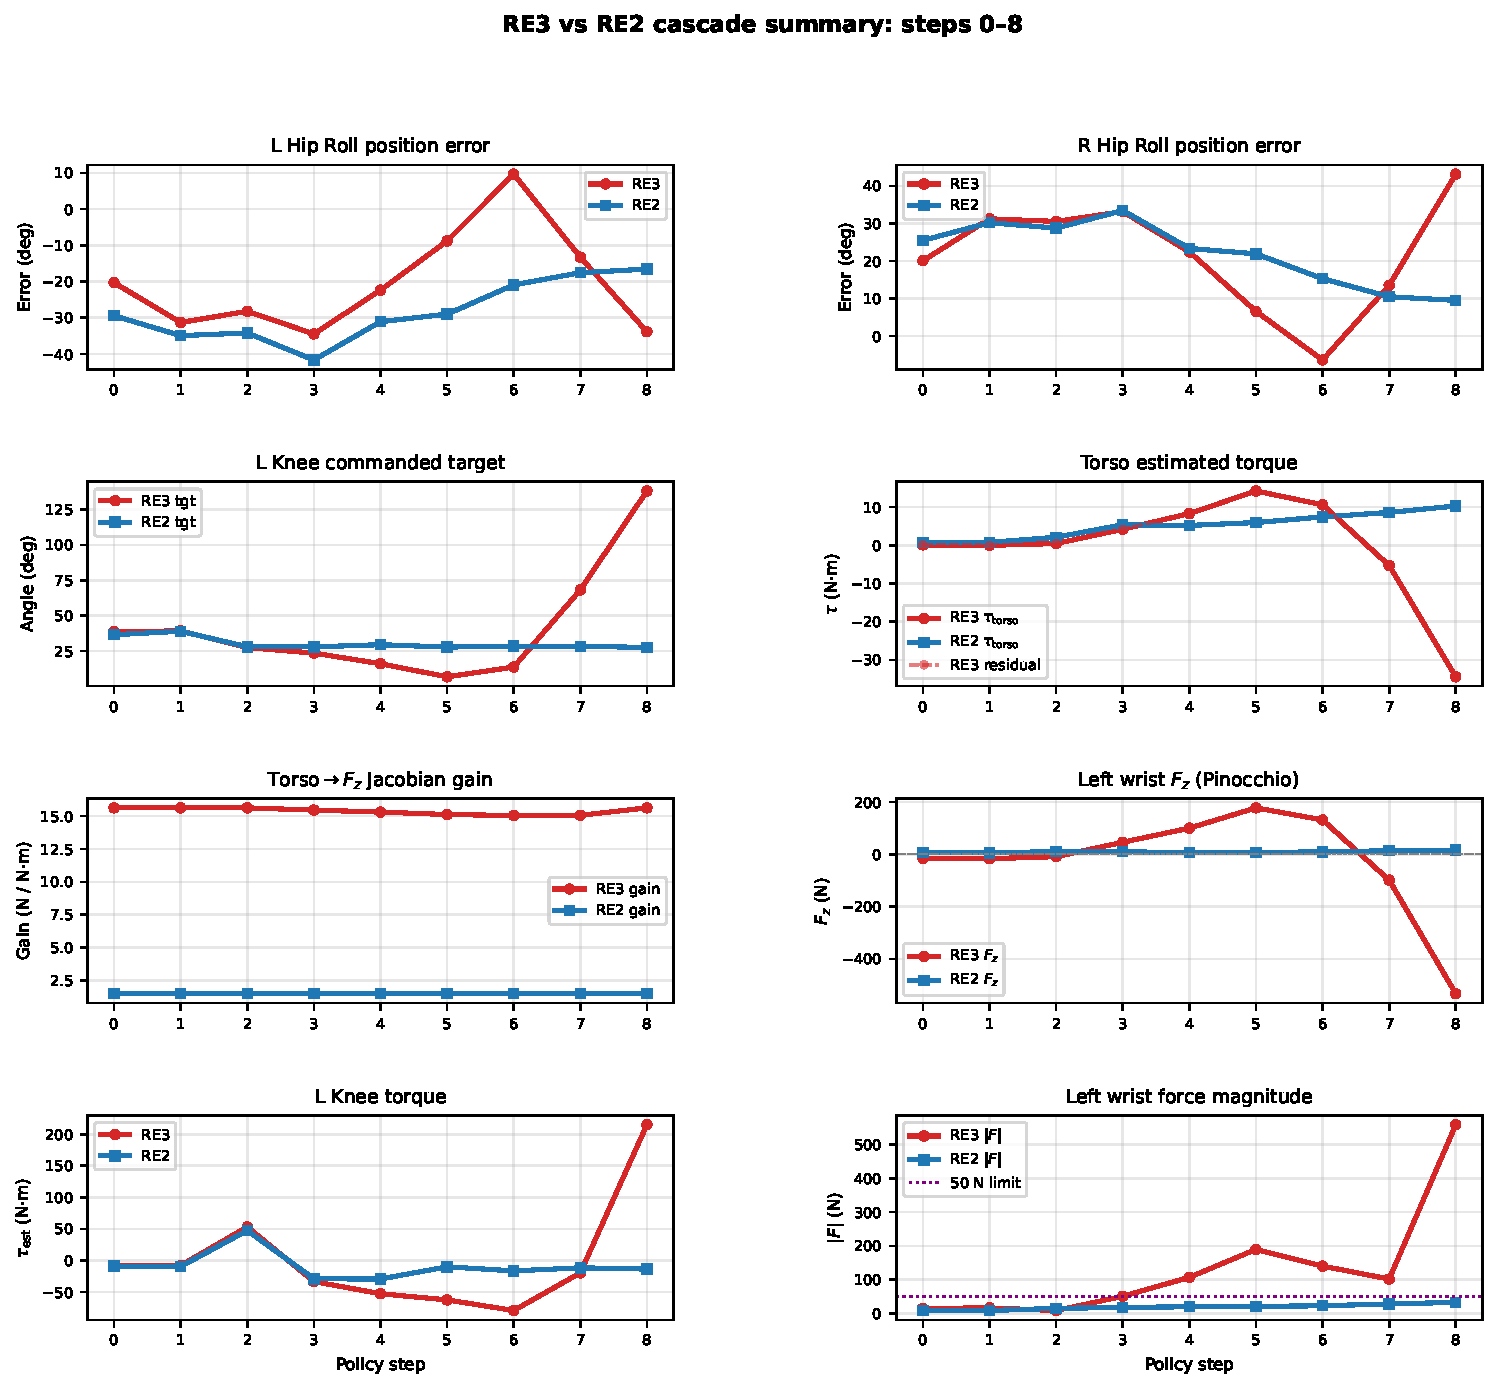
\includegraphics[width=\textwidth]{figures/fig_cascade_summary.pdf}
  \caption{All key quantities for RE2 (blue) and RE3 (red), steps 0--8,
           in a single panel.  Reading top-to-bottom, left-to-right: hip
           roll errors (comparable for both); knee commanded targets
           (diverge sharply in RE3 from step 7); torso torque (grows in
           both, but RE3 spikes harder); torso Jacobian gain (flat 15.6
           for RE3, flat 1.5 for RE2); wrist Fz (explosive in RE3); wrist
           force magnitude (exceeds 100 N in RE3 by step 4).}
  \label{fig:cascade_summary}
\end{figure}

% ═════════════════════════════════════════════════════════════════════════════
\section{The Torso as a Kinematic Junction: Unavoidable Contamination}
% ═════════════════════════════════════════════════════════════════════════════

\subsection{Why Torso Torque Is Never Zero During a Real Run}

Equation~\eqref{eq:wrench_estimator} assumes the sole source of torque
residual is an external wrench at the wrist.  In any real deployment this
assumption is structurally violated because the torso joint sits at a
\emph{kinematic junction}: the legs (with ground-contact forces below) and
the arms (to be estimated above) both connect to it.

Even in a nominally stationary standing pose, the robot is never in perfect
bilateral stance.  The leg joints are slightly bent, the CoM may be
marginally offset, and the ground-contact forces at the left and right feet
are unequal.  These real external wrenches at the feet propagate up the
leg kinematic chain and appear as residual torques at every joint from the
ankles to the torso:
\begin{equation}
  \tau_\text{torso}^\text{res}
  = \underbrace{\tau_{\text{feet}\to\text{torso}}}_{\text{ground-contact coupling}}
  + \underbrace{\tau_\text{inertial}}_{\text{dynamic loading}}
  + \underbrace{\tau_\text{friction}}_{\text{joint friction}}
  - \underbrace{0}_{\tau_\text{grav,torso} \approx 0 \text{ at upright}}.
  \label{eq:torso_res_sources}
\end{equation}
None of these contributions has anything to do with an external force at
the wrist.  The wrench estimator, however, cannot distinguish them: it
projects everything in $\btau_\text{res}$ onto the wrist frame via
$\pinv{(\bJ^T)}$.

\begin{figure}[H]
  \centering
  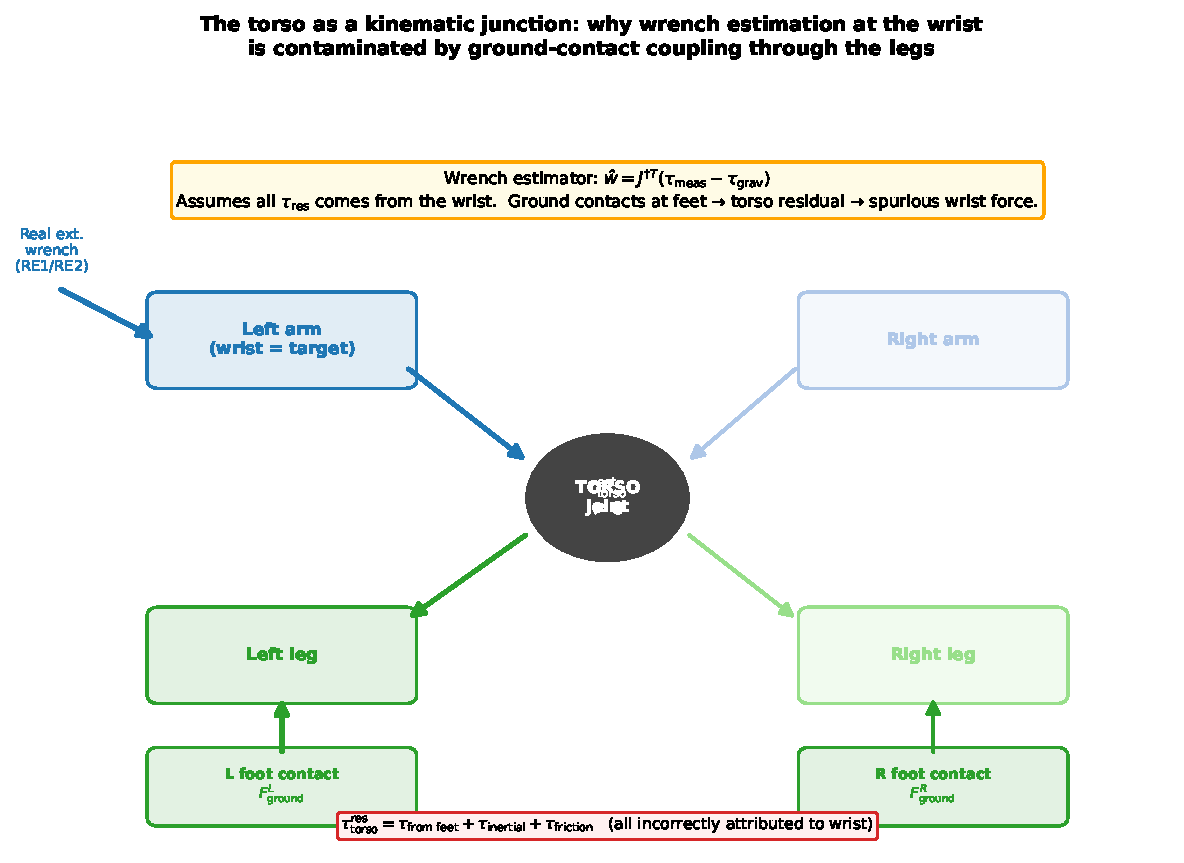
\includegraphics[width=0.80\textwidth]{figures/fig_kinematic_junction.pdf}
  \caption{The torso joint connects the lower body (legs, feet, ground
           contacts) with the upper body (arms, wrist).  Ground-contact
           wrenches at the feet propagate up through the leg kinematic
           chain and produce a non-zero torso torque residual that the
           wrench estimator incorrectly attributes to an external load at
           the wrist.  The fundamental ambiguity cannot be resolved without
           a separate model for foot contact.}
  \label{fig:kinematic_junction}
\end{figure}

\subsection{RE1/RE2: Torso Residual Always Present, Never Catastrophic}

Full-run Pinocchio analysis of RE1 (2620 steps) and RE2 (1357 steps)
confirms this contamination is a persistent feature, not an anomaly:

\begin{table}[H]
\centering
\caption{Torso joint torque statistics over complete successful runs.}
\label{tab:torso_stats}
\begin{tabular}{lrrrr}
\toprule
Episode & Mean $|\tau_\text{torso}|$ & Std & Max $|\tau_\text{torso}|$ & p99 \\
        & (N$\cdot$m) & (N$\cdot$m) & (N$\cdot$m) & (N$\cdot$m) \\
\midrule
\good{RE1 (2620 steps)} & 1.6 & 0.9 & 11.3 & 4.0 \\
\good{RE2 (1357 steps)} & 0.8 & 1.4 & 10.5 & 6.6 \\
\bottomrule
\end{tabular}
\end{table}

At the RE1/RE2 Jacobian gain of $\approx$1.5, these torso residuals
produce wrist-force contamination of only $\sim$1--2\,N on average and
$\sim$14\,N at the worst.  This is swamped by the actual external loads
the experimenter is applying to the arms during those runs, so the
estimator still delivers a reasonable (though noisy) measurement.

\subsection{Why RE1/RE2 Wrist Forces Track the Real Load, Not the Torso}

In RE1 and RE2, the experimenter is actively applying real forces to the
robot's wrists during the run.  These real wrenches are transmitted through
the arm joints to the torso: the arm motors must exert torques to counteract
the external load.  The resulting arm-joint residuals are large compared
with the torso contamination, and the wrench estimator correctly attributes
most of the signal to a wrist load:

\begin{equation}
  \hat\bw \approx
    \underbrace{\text{arm-joint contribution}}_{\text{large, real}}
  + \underbrace{\text{torso contribution}}_{\text{small: gain }1.5\times r_\text{torso}}.
\end{equation}

In RE3, there is no real external wrist load.  The arm-joint residuals
are near zero (the arms are free-hanging), leaving only the torso
contamination.  With gain 15.6, this contamination dominates:
\begin{equation}
  \hat{F}_z^{\text{RE3}} \approx \underbrace{15.6 \times (-34.5)}_{\text{torso}}
  + \underbrace{(\text{arm terms})}_{\approx +7\,\text{N}}
  = -532\,\text{N}.
\end{equation}

\subsection{Hypothetical: RE1/RE2 Arm Config Counterfactual}

Had RE1 or RE2 been run with the arms in the RE3 extended pose, the
\emph{same torso residuals} they already exhibited would have produced
catastrophically large spurious wrist forces.  With gain 15.6 and
max torso residual $\approx$9\,N$\cdot$m:
\begin{equation}
  |F_z|_\text{hypothetical} = 15.6 \times 9\,\text{N}\cdot\text{m}
  = 140\,\text{N} \quad \text{(from torso alone)}.
\end{equation}
This is well above the 50\,N threshold that triggered catastrophic
leg commands in RE3.

\begin{figure}[H]
  \centering
  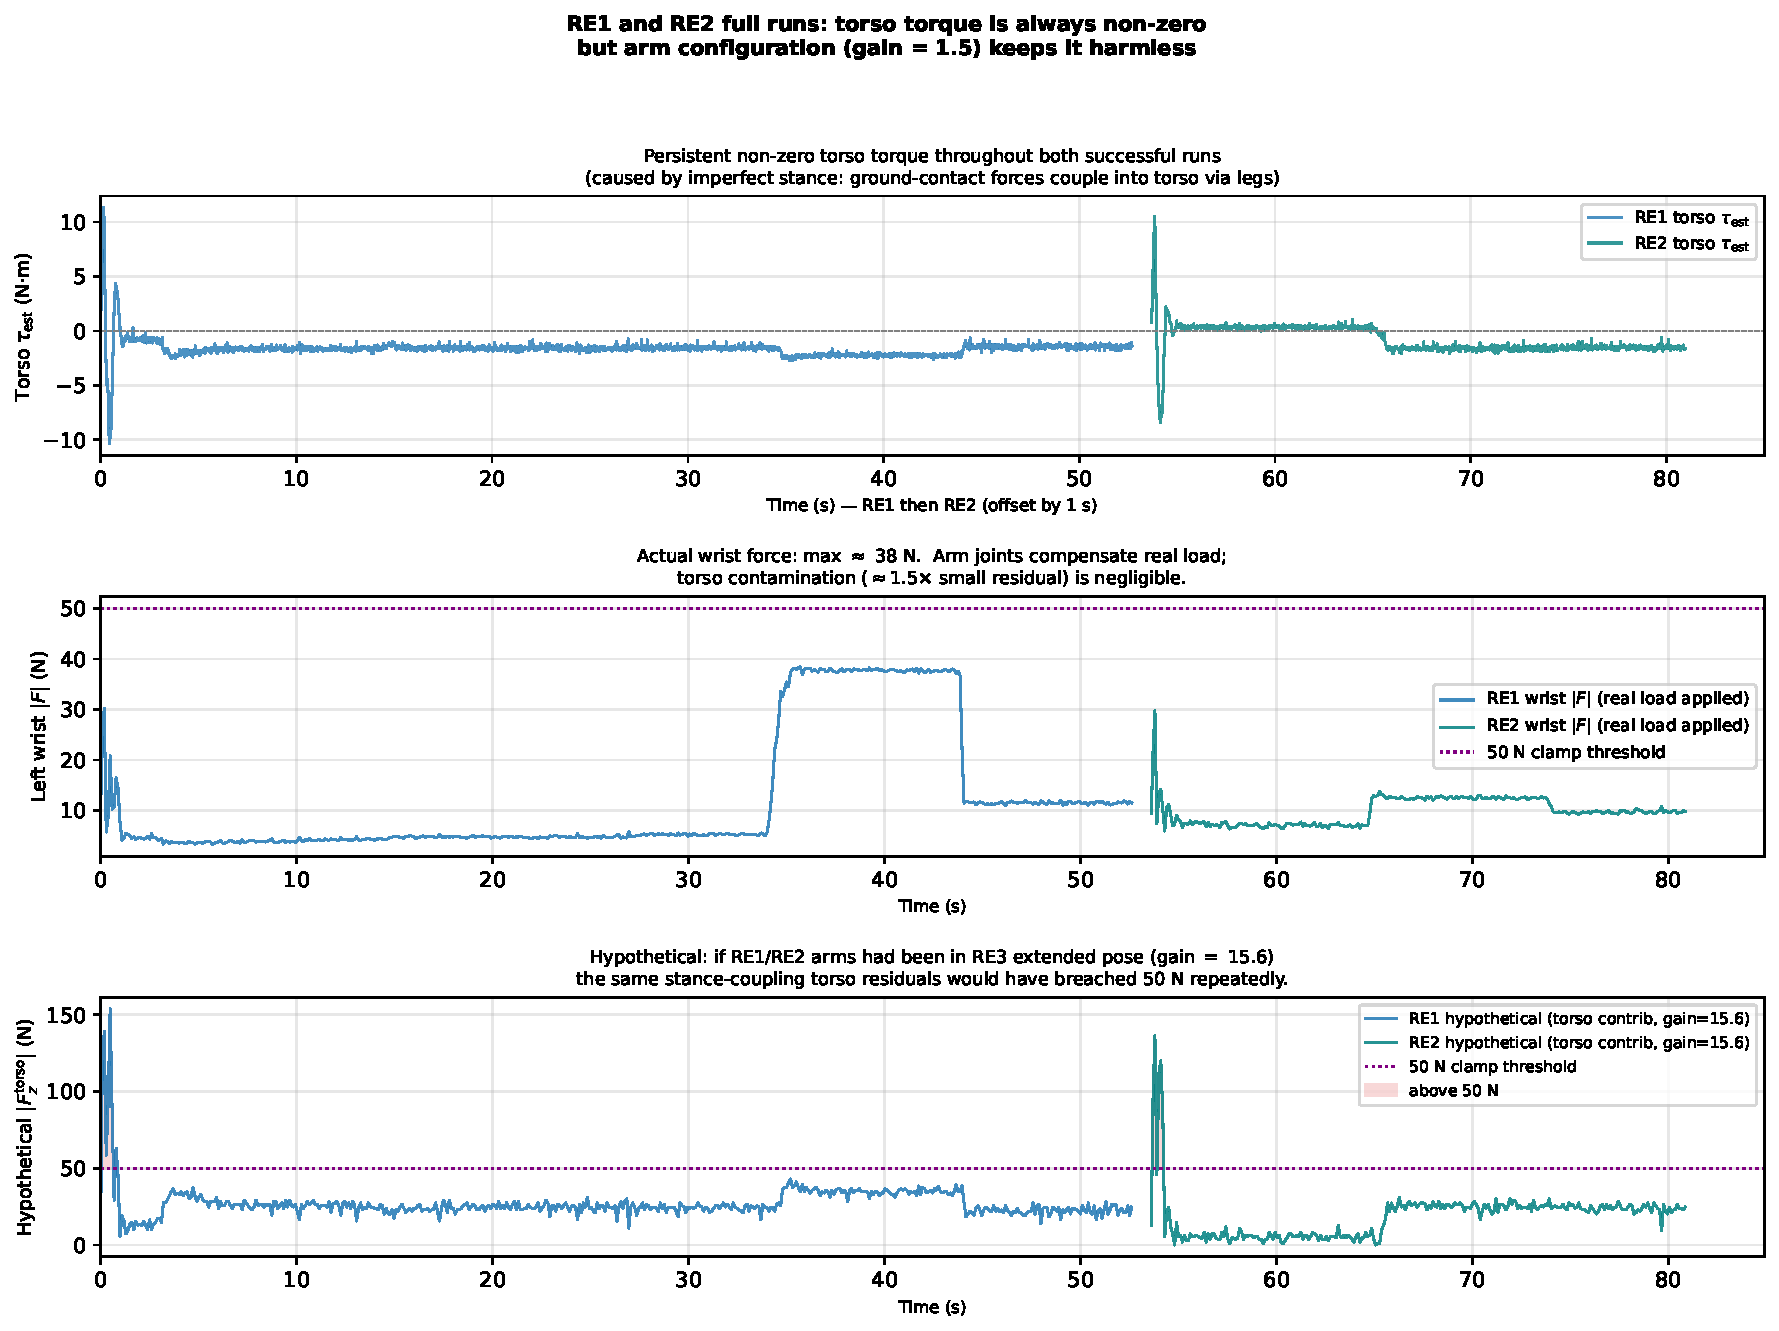
\includegraphics[width=\textwidth]{figures/fig_re1re2_full_run.pdf}
  \caption{\emph{Top}: torso estimated torque throughout the complete RE1
           and RE2 runs.  The torso is never at zero; the mean is
           $-$1.6\,N$\cdot$m with excursions to $\pm$11\,N$\cdot$m,
           driven by stance-coupling from imperfect bilateral ground
           contact.
           \emph{Middle}: actual left wrist $|F|$ stays below 38\,N
           throughout both runs.  The arm joints are compensating real
           applied loads; the torso contamination is negligible at gain = 1.5.
           \emph{Bottom}: hypothetical wrist force if the arms had been in
           the RE3 extended pose (gain = 15.6, torso contribution only).
           The same stance residuals would have repeatedly exceeded 50\,N
           (shaded red), enough to trigger the same destabilising feedback
           loop.}
  \label{fig:re1re2_full}
\end{figure}

\subsection{The Fundamental Indistinguishability}

A real wrist force \emph{does} drive a torso torque: the arm motor chain
transmits external loads back toward the base, and the torso motor must
resist some of that reaction.  So the torso torque residual is not
purely noise---it is partially signal.  The fundamental problem is
\emph{indistinguishability}: the torso's $\tau_\text{res}$ is a
superposition of all external loads attached to its kinematic tree:

\begin{equation}
  \btau_\text{res} = \bJ_{\text{L-wrist}}^T \bw_{\text{L-wrist}}
                   + \bJ_{\text{R-wrist}}^T \bw_{\text{R-wrist}}
                   + \bJ_{\text{L-foot}}^T \bw_{\text{L-foot}}
                   + \bJ_{\text{R-foot}}^T \bw_{\text{R-foot}}
                   + \btau_\text{inertial}.
  \label{eq:full_budget}
\end{equation}

Projecting through $\pinv{(\bJ_\text{wrist}^T)}$ recovers
$\bw_\text{wrist}$ exactly only if the foot and inertial terms are zero.
When a real wrist load is present and large, it dominates the torso
residual and the estimate is approximately correct (RE1/RE2).  When there
is \emph{no} real wrist load, the foot-coupling and inertial terms are
the only contributors, and the estimator attributes all of them to an
imaginary wrist force.  The torso's Jacobian gain then determines whether
this error is negligible (gain = 1.5, RE1/RE2 pose) or catastrophic
(gain = 15.6, RE3 arm-extended pose).

% ═════════════════════════════════════════════════════════════════════════════
\section{Discussion}
% ═════════════════════════════════════════════════════════════════════════════

\subsection{Original vs.\ Revised Hypothesis}

The original investigation framed the disaster as a spurious Pinocchio
force causing a leg reaction.  This was correct in direction but incomplete
in mechanism.  A cleaner framing:

\begin{quote}
\textit{The robot's own structural dynamics (normal leg PD corrections) drove
a real torso torque of $-34$\,N$\cdot$m by step 8.  Under a
well-conditioned Jacobian (RE2, gain 1.5), this is invisible ($\to$ 15\,N
wrist force).  Under the ill-conditioned Jacobian set by the
\texttt{arm\_waist\_target} pose (RE3, gain 15.6), the same torso torque
becomes a $-532$\,N phantom wrist force, which the RL policy then
desperately and destructively tries to counteract.}
\end{quote}

\noindent The wrench is spurious, but it originates from a real mechanical
event (the torso joint fighting structural reaction forces), not from a
numerical bug or modelling error.  The amplification is geometric,
determined entirely by the arm pose at wrench estimation time.

\subsection{Why the Arms Were in the Bad Pose}

The \texttt{arm\_waist\_target} pose is defined in the deploy configuration:
\begin{lstlisting}
arm_waist_target = [0.0,              # torso
                    -0.3, 0.0, 0.0, 1.5, 0.0, 0.0, 0.0,   # left arm
                    -0.9, -0.47, 0.0, 0.5, 0.0, 0.0, 0.0]  # right arm
\end{lstlisting}
This places the left shoulder pitch at $-0.3$ rad ($-17^\circ$ from motor
zero) and the left elbow at $1.5$ rad ($+86^\circ$ from motor zero, which
physically rotates the forearm $86^\circ$ from the bent-at-sides reference,
extending the arm nearly straight down).  The right arm is in a different
non-zero offset (shoulder pitched $-52^\circ$, rolled inward, elbow at
$+30^\circ$ from zero) --- this partly extends it but in a different
direction, keeping the right wrist at a higher $z$ position than the left
and resulting in a lower (though still elevated) Jacobian gain for the right
wrist.  This is consistent with why the right wrist force in RE3 did not
show the same explosion as the left.

The intent of \texttt{arm\_waist\_target} is presumably to position the
hands near the robot's waist for future manipulation tasks.  However, this
configuration was never tested for compatibility with the
wrench-conditioned RL policy.

\subsection{Why RE1 and RE2 Were Safe}

As shown in Table~\ref{tab:arm_range} and Figure~\ref{fig:gain_vs_angle},
RE1 and RE2 ran with arms remaining at motor zero ($<5^\circ$ variation
throughout entire thousands-of-step runs).  Motor zero on the H1.2
physically corresponds to forearms bent at the sides --- a compact,
well-conditioned arm pose with Jacobian gain $\approx 1.5$.

The arms never moved during these runs because the RL policy has no arm
action outputs: arm positions are held at whatever initial configuration
is set by the deploy script.  In RE1/RE2 that configuration was motor zero
(bent at sides); in RE3 it was \texttt{arm\_waist\_target} (left arm
extended downward).

At gain $\approx 1.5$, even RE2's peak torso residual of 10.3 N$\cdot$m
only produces 15.8\,N of apparent wrist force---well below any real
load threshold.

\subsection{Implications}

\begin{enumerate}
\item \textbf{Arm pose is a safety-critical parameter} for the wrench
      estimator.  Any deployment that uses a non-default arm configuration
      must verify the resulting torso-to-wrist Jacobian gain is acceptable
      ($<3$ N/N$\cdot$m recommended).

\item \textbf{The wrench estimator's assumption is fundamentally violated
      in full-body motion.}  The assumption $\btau_\text{res} = \bJ^T\bw$
      (Eq.~\ref{eq:static_eq}) is a static approximation.  During dynamic
      whole-body motion, inertial and Coriolis torques are the dominant
      residuals, and they have nothing to do with external forces at the
      wrist.

\item \textbf{A hard output clamp would have prevented this disaster.}
      Had the wrench output been clamped to $|\bm{F}| < 50$\,N before
      passing to the encoder, step 3's 46\,N would have been truncated and
      the policy never received damaging feedback.
\end{enumerate}

% ═════════════════════════════════════════════════════════════════════════════
\section{Recommendations}
% ═════════════════════════════════════════════════════════════════════════════

Table~\ref{tab:recs_summary} gives a one-line summary of each recommendation;
the subsections below develop the math and intuition for each.

\begin{table}[H]
\centering
\caption{Prioritised recommendations (detailed in subsections below).}
\label{tab:recs_summary}
\begin{tabular}{clll}
\toprule
Priority & \S & Type & One-line summary \\
\midrule
\textbf{Critical} & \ref{sec:rec_clamp}   & Output clamp & $\pm 50$\,N hard clip before passing to encoder \\
\textbf{Critical} & \ref{sec:rec_preflight} & Pre-flight & Check Jacobian gain $<3$ and initial hip error $<0.15$\,rad \\
\textbf{High}     & \ref{sec:rec_stacked}  & Better estimator & Stacked 4-endpoint estimator; explicitly models foot contacts \\
\textbf{High}     & \ref{sec:rec_armcheck} & Sanity check & Arm-vs-torso residual ratio flags structural contamination \\
\textbf{High}     & \ref{sec:rec_imu}      & Gravity comp. & Pass IMU quaternion to \texttt{get\_frame\_wrench} \\
\textbf{Medium}   & \ref{sec:rec_condnum}  & Monitor & Log Jacobian condition number; disable if $\kappa>20$ \\
\textbf{Medium}   & \ref{sec:rec_watchdog} & Watchdog & Disengage policy if $|\bm{F}|>100$\,N for $>3$ steps \\
\bottomrule
\end{tabular}
\end{table}

% ─────────────────────────────────────────────────────────────────────────────
\subsection{R1. Output Clamp (Immediate, One Line of Code)}
\label{sec:rec_clamp}

Add a hard magnitude clamp to \texttt{get\_frame\_wrench} before returning:
\begin{lstlisting}
wrench = np.linalg.pinv(jac.T) @ (tau - tau_gravity)
wrench[:3] = np.clip(wrench[:3], -F_max, F_max)   # add this
return wrench
\end{lstlisting}
with $F_\text{max} = 50$\,N as a conservative starting point.  This would
have completely prevented the RE3 disaster: the first out-of-bound estimate
($F_z = +46$\,N) would have been clipped at step 3, and the policy would
never have received damaging feedback.

50\,N is intentionally conservative.  The RL policy was trained with wrist
forces in the range the experimenter could apply by hand; anything larger
almost certainly reflects the estimator breakdown described in this report.
As the estimator is improved (see \S\ref{sec:rec_stacked}), $F_\text{max}$
can be raised.

% ─────────────────────────────────────────────────────────────────────────────
\subsection{R2. Pre-flight Safety Checks}
\label{sec:rec_preflight}

Two checks before engaging the RL policy:

\subsubsection*{Check A: Jacobian condition / torso gain}
Compute the torso$\to$wrist-$F_z$ gain at the current arm pose:
\begin{lstlisting}
J    = robot_model.get_frame_jacobian("left_wrist_yaw_link", q)
JpTi = np.linalg.pinv(J.T)
g    = abs(JpTi[2, 12])   # torso column, Fz row (index 12 = torso)
assert g < 3.0, f"Jacobian gain too high: {g:.1f} N/(N*m)"
\end{lstlisting}
At motor zero (arms bent at sides) $g \approx 1.5$.  As shown in
Figure~\ref{fig:gain_vs_angle}, the gain rises sharply as the elbow extends;
the threshold of 3\,N/N$\cdot$m gives comfortable margin.

\subsubsection*{Check B: Initial lower-body configuration}
Assert that hip-roll deviations are within tolerance before policy start:
\begin{lstlisting}
for j, name in [(2, "l_hip_roll"), (8, "r_hip_roll")]:
    err = abs(qpos[j] - target_dof[j])
    assert err < 0.15, f"{name} start error {np.degrees(err):.1f} deg"
\end{lstlisting}
Large initial hip-roll errors ($>0.15$\,rad, $>9^\circ$) cause immediate
large PD torques that excite the torso and amplify whatever gain is present.

% ─────────────────────────────────────────────────────────────────────────────
\subsection{R3. Stacked Multi-Endpoint Estimator}
\label{sec:rec_stacked}

\subsubsection*{Motivation}
The current estimator projects all of $\btau_\text{res}$ onto a single
endpoint.  As Eq.~\eqref{eq:full_budget} shows, the residual actually
contains contributions from both wrists and both feet.  When only the wrist
is modelled, the foot terms contaminate the estimate.

\subsubsection*{Math}
Define the \emph{stacked contact Jacobian} for all four endpoints:
\begin{equation}
  A \triangleq
  \begin{bmatrix}
    \bJ_{\text{L-wrist}}^T &
    \bJ_{\text{R-wrist}}^T &
    \bJ_{\text{L-foot}}^T &
    \bJ_{\text{R-foot}}^T
  \end{bmatrix}
  \in \R{n_v \times 24},
  \label{eq:A_stack}
\end{equation}
where each $\bJ_i^T \in \R{n_v \times 6}$ and $n_v = 27$.  The stacked
wrench vector is $\bm{w}_\text{all} = [\bw_\text{Lw};\, \bw_\text{Rw};\,
\bw_\text{Lf};\, \bw_\text{Rf}] \in \R{24}$.  Under the same static
equilibrium assumption as Eq.~\eqref{eq:static_eq}:
\begin{equation}
  \btau_\text{res} = A\,\bm{w}_\text{all},
  \label{eq:stacked_sys}
\end{equation}
which is now a $27 \times 24$ \emph{overdetermined} system (more equations
than unknowns).  The minimum-norm least-squares solution is:
\begin{equation}
  \hat{\bm{w}}_\text{all} = \pinv{A}\,\btau_\text{res},
  \quad \pinv{A} \in \R{24 \times 27}.
  \label{eq:stacked_sol}
\end{equation}
The first six components are $\hat\bw_\text{L-wrist}$; the next six
$\hat\bw_\text{R-wrist}$; the last twelve the foot wrenches.

\subsubsection*{Why this helps}
In the overdetermined system, if the foot-contact columns of $A$ can
explain a torque residual, the least-squares fit assigns it to a foot
wrench rather than a wrist wrench.  The torso residual arising from
imperfect stance (always present, as shown in \S\ref{sec:re1re2_arms}) is
naturally absorbed by the foot-contact terms, removing it from the wrist
estimate.

Concretely: in the single-endpoint estimator, a torso residual of
$-34.5$\,N$\cdot$m was projected entirely into $F_z^\text{L-wrist}$
(gain 15.6, giving $-539$\,N).  In the stacked estimator, the foot
Jacobian columns provide an alternative explanation (the robot is leaning
slightly, the ground is pushing back) and the residual is partitioned
across wrist and foot estimates.  The wrist term is dramatically smaller.

\subsubsection*{Implementation}
\begin{lstlisting}
frames = ["left_wrist_yaw_link", "right_wrist_yaw_link",
          "left_ankle_roll_link", "right_ankle_roll_link"]
Jcols  = [robot_model.get_frame_jacobian(f, q) for f in frames]
A      = np.hstack([J.T for J in Jcols])     # 27 x 24
w_all  = np.linalg.lstsq(A, tau_res, rcond=None)[0]   # 24,
w_left_wrist  = w_all[0:6]
w_right_wrist = w_all[6:12]
\end{lstlisting}
Using \texttt{lstsq} (backed by a QR decomposition) rather than
\texttt{pinv} is numerically preferable for the overdetermined case.
The condition number of $A$ is typically much lower than that of
$\bJ_\text{wrist}$ alone, because foot-contact Jacobians fill in
the null-space directions.

\subsubsection*{Limitation}
The stacked estimator still makes the static equilibrium assumption and
does not model inertial torques.  It is a better approximation at low
speeds; for highly dynamic motions a full inverse dynamics model is
needed.  The clamp in \S\ref{sec:rec_clamp} should remain as a backstop.

% ─────────────────────────────────────────────────────────────────────────────
\subsection{R4. Arm-vs-Torso Residual Consistency Check}
\label{sec:rec_armcheck}

\subsubsection*{Intuition}
A real external force at the wrist must travel through the arm kinematic
chain before reaching the torso.  The joints closest to the wrist---elbow,
shoulder---must each exert torque to transmit the load.  If the wrist force
estimate is large but the arm joints show no corresponding torque residual,
the estimate is almost certainly driven by structural contamination rather
than a real force.

In the RE1/RE2 healthy runs, arm joint residuals dominated the wrist force
estimate (mean arm contribution $\approx 12$\,N at wrist, torso contribution
$\approx 2$\,N).  In RE3, the reverse was true at step 8: arm residual norm
was only $\sim$1.6\,N$\cdot$m while the torso alone generated $-538$\,N.

\subsubsection*{Math}
Partition the residual and Jacobian into arm columns (indices 13--26,
excluding torso) and the torso column (index 12):
\begin{align}
  \hat\bw_\text{arm}   &= \pinv{(\bJ^T)}\,_{[:,\,13:26]}\;
                          \btau_\text{res}[13:26], \\
  \hat\bw_\text{torso} &= \pinv{(\bJ^T)}\,_{[:,\,12]}\;
                          \btau_\text{res}[12].
\end{align}
Define the \emph{torso dominance ratio}:
\begin{equation}
  \rho \triangleq
  \frac{|\hat{F}_{z,\,\text{torso}}|}
       {|\hat{F}_{z,\,\text{torso}}| + \|\hat\bw_\text{arm}[:3]\| + \varepsilon}.
  \label{eq:rho}
\end{equation}
When a real wrist load is present, arm joints carry the bulk of the signal
and $\rho \ll 1$.  When the estimate is dominated by structural contamination
(as in RE3 step 8: $|\hat{F}_{z,\text{torso}}| = 538$\,N vs arm $= 7$\,N),
$\rho \to 1$.

\subsubsection*{Implementation}
\begin{lstlisting}
JpTinv    = np.linalg.pinv(jac.T)          # 6 x 27
res       = tau - tau_gravity

arm_idx   = list(range(13, 27))
torso_idx = 12

Fz_torso  = JpTinv[2, torso_idx] * res[torso_idx]
Fz_arm    = np.linalg.norm(JpTinv[2, arm_idx] * res[arm_idx])
rho       = abs(Fz_torso) / (abs(Fz_torso) + Fz_arm + 1e-6)

if rho > 0.5:   # torso drives >50% of the Fz estimate
    wrench = np.zeros(6)   # zero out or clamp
    log_warning(f"High torso dominance (rho={rho:.2f}); zeroing wrench estimate")
\end{lstlisting}

A threshold of $\rho > 0.5$ is conservative; at step 8 in RE3 the ratio is
$538 / (538 + 7) = 0.99$.  In the healthy RE1/RE2 runs, $\rho$ stays
below 0.2 throughout.

Note that $\rho$ is configuration-dependent as well as signal-dependent:
it is high either because the Jacobian gain is large (arm pose) or because
arm joints are genuinely quiet (no real load).  Combining this check with
the pre-flight Jacobian gain check (\S\ref{sec:rec_preflight}) gives a
cleaner signal.

% ─────────────────────────────────────────────────────────────────────────────
\subsection{R5. IMU-Corrected Gravity Compensation}
\label{sec:rec_imu}

The current \texttt{get\_frame\_wrench} defaults to an identity base
orientation when \texttt{imu\_quat} is not supplied.  During dynamic
whole-body motion, the pelvis tilts and the gravity vector as seen in the
pelvis frame rotates, adding a systematic error to $\btau_\text{grav}$:
\begin{equation}
  \delta\btau_\text{grav} \approx \frac{\partial \btau_\text{grav}}{\partial\phi}
  \cdot \phi_\text{tilt},
\end{equation}
where $\phi_\text{tilt}$ is the pelvis tilt angle.  For a $5^\circ$ tilt
and a robot with total mass $\sim 47$\,kg this adds $\sim$5--10\,N$\cdot$m
of spurious residual across the upper-body joints.  At gain 15.6, this
translates to 78--156\,N of additional phantom wrist force.

Fix: always pass the IMU quaternion:
\begin{lstlisting}
wrench = robot_model.get_frame_wrench(
    "left_wrist_yaw_link",
    q=q, tau=tau, imu_quat=imu_state.quaternion)
\end{lstlisting}

% ─────────────────────────────────────────────────────────────────────────────
\subsection{R6. Jacobian Condition Number Monitor}
\label{sec:rec_condnum}

The condition number $\kappa = \sigma_\text{max}/\sigma_\text{min}$ of
$\bJ_\text{wrist}$ is a direct measure of how amplified any residual
direction will be.  It can be computed cheaply from the SVD already required
for the pseudo-inverse:
\begin{lstlisting}
_, S, _ = np.linalg.svd(jac)
kappa   = S[0] / S[-1]
if kappa > 20:
    log_warning(f"Wrist Jacobian ill-conditioned: kappa={kappa:.1f}")
    # optionally disable wrench input to encoder
\end{lstlisting}
In all healthy configurations observed, $\kappa < 15$ (RE1/RE2: $\approx$13).
RE3's initial $\kappa = 39.9$ would have triggered this check at episode
start.  A threshold of 20 gives safe margin while allowing moderate arm
poses.

% ─────────────────────────────────────────────────────────────────────────────
\subsection{R7. Real-Time Watchdog}
\label{sec:rec_watchdog}

Even with all the above in place, a runtime guard provides a final safety
layer.  Track a consecutive-exceedance counter:
\begin{lstlisting}
FORCE_LIMIT   = 100.0   # N
CONSEC_THRESH = 3       # steps (~60 ms at 50 Hz)

if np.linalg.norm(wrench[:3]) > FORCE_LIMIT:
    consec_count += 1
else:
    consec_count = 0

if consec_count >= CONSEC_THRESH:
    policy.disengage()
    robot.enter_damping_mode()
\end{lstlisting}
This catches any failure mode not addressed by the estimator improvements,
including transient hardware faults or unseen policy pathologies.  The
100\,N / 3-step threshold gives 60\,ms of response time---fast enough to
prevent significant damage.

% ═════════════════════════════════════════════════════════════════════════════
\section{Conclusions}
% ═════════════════════════════════════════════════════════════════════════════

The RE3 disaster was caused by a single configuration parameter:
\texttt{arm\_waist\_target} placed the robot's arms in a raised, bent pose
that created a 15.6$\times$ amplification of the torso joint's torque
residual into an apparent wrist force.  Normal structural dynamics---the
torso motor fighting inertial reaction forces from the legs---produced a
torso residual that, under this amplification, became a $-532$\,N phantom
external push at the left wrist.  The RL policy responded as trained:
with large leg forces to counteract a large external load.

RE1 and RE2 avoided this failure not because their leg dynamics were
gentler, but because their arms never left the natural hanging position
($< 5^\circ$ throughout entire multi-thousand-step runs), keeping the
Jacobian gain at a benign 1.5.

The fundamental lesson is that the Pinocchio wrench estimator
(\texttt{pinv(J\^{}T) @ tau\_residual}) has a hidden configuration
dependency: its accuracy degrades as the arm moves into poses that are
kinematically far from the natural hang, and this degradation is
catastrophic in combination with a policy that receives the wrench estimate
directly as input.

\bigskip
\noindent\textbf{The single most impactful fix} is adding a
$\pm 50$\,N output clamp to \texttt{get\_frame\_wrench}.  This requires
one line of code and would have completely prevented the RE3 incident.

\appendix
% ═════════════════════════════════════════════════════════════════════════════
\section{Data Provenance and Reproducibility}
% ═════════════════════════════════════════════════════════════════════════════

\begin{table}[H]
\centering
\caption{Episode data files used in this analysis.}
\begin{tabular}{lll}
\toprule
Episode & Path & Steps \\
\midrule
RE3 (disaster) & \texttt{data/real/re3\_real\_encode\_tr1/} & 77 \\
RE2 (good)     & \texttt{data/real/re2\_real\_encode/}     & 1357 \\
RE1 (good)     & \texttt{data/real/re1\_real\_encode/}     & 2620 \\
\bottomrule
\end{tabular}
\end{table}

All Pinocchio calculations use the H1.2 URDF at:\\
\texttt{ws\_ctrl/src/h12\_ros2\_controller/assets/h1\_2/h1\_2\_handless.urdf}

To regenerate all figures:
\begin{lstlisting}[language=bash, caption={Reproduce figures.}]
/home/humanoid/Programs/h12_ros2_controller/.venv/bin/python \
    docs/generate_re3_figures.py
\end{lstlisting}

To compile this document (requires TeX Live / pdflatex):
\begin{lstlisting}[language=bash, caption={Compile LaTeX.}]
cd docs && pdflatex re3_root_cause_analysis.tex
\end{lstlisting}

\begin{thebibliography}{9}
\bibitem{pinocchio}
  J.\ Carpentier, G.\ Saurel, G.\ Buondonno, J.\ Mirabel, F.\ Lamiraux,
  O.\ Stasse, N.\ Mansard.
  ``The Pinocchio C++ library: A fast and flexible implementation of rigid
  body dynamics algorithms and their analytical derivatives.''
  \textit{IEEE SYROCO}, 2019.
\end{thebibliography}

\end{document}
